% Options for packages loaded elsewhere
\PassOptionsToPackage{unicode}{hyperref}
\PassOptionsToPackage{hyphens}{url}
%
\documentclass[
]{article}
\usepackage{amsmath,amssymb}
\usepackage{lmodern}
\usepackage{iftex}
\ifPDFTeX
  \usepackage[T1]{fontenc}
  \usepackage[utf8]{inputenc}
  \usepackage{textcomp} % provide euro and other symbols
\else % if luatex or xetex
  \usepackage{unicode-math}
  \defaultfontfeatures{Scale=MatchLowercase}
  \defaultfontfeatures[\rmfamily]{Ligatures=TeX,Scale=1}
\fi
% Use upquote if available, for straight quotes in verbatim environments
\IfFileExists{upquote.sty}{\usepackage{upquote}}{}
\IfFileExists{microtype.sty}{% use microtype if available
  \usepackage[]{microtype}
  \UseMicrotypeSet[protrusion]{basicmath} % disable protrusion for tt fonts
}{}
\makeatletter
\@ifundefined{KOMAClassName}{% if non-KOMA class
  \IfFileExists{parskip.sty}{%
    \usepackage{parskip}
  }{% else
    \setlength{\parindent}{0pt}
    \setlength{\parskip}{6pt plus 2pt minus 1pt}}
}{% if KOMA class
  \KOMAoptions{parskip=half}}
\makeatother
\usepackage{xcolor}
\usepackage[margin=1in]{geometry}
\usepackage{longtable,booktabs,array}
\usepackage{calc} % for calculating minipage widths
% Correct order of tables after \paragraph or \subparagraph
\usepackage{etoolbox}
\makeatletter
\patchcmd\longtable{\par}{\if@noskipsec\mbox{}\fi\par}{}{}
\makeatother
% Allow footnotes in longtable head/foot
\IfFileExists{footnotehyper.sty}{\usepackage{footnotehyper}}{\usepackage{footnote}}
\makesavenoteenv{longtable}
\usepackage{graphicx}
\makeatletter
\def\maxwidth{\ifdim\Gin@nat@width>\linewidth\linewidth\else\Gin@nat@width\fi}
\def\maxheight{\ifdim\Gin@nat@height>\textheight\textheight\else\Gin@nat@height\fi}
\makeatother
% Scale images if necessary, so that they will not overflow the page
% margins by default, and it is still possible to overwrite the defaults
% using explicit options in \includegraphics[width, height, ...]{}
\setkeys{Gin}{width=\maxwidth,height=\maxheight,keepaspectratio}
% Set default figure placement to htbp
\makeatletter
\def\fps@figure{htbp}
\makeatother
\setlength{\emergencystretch}{3em} % prevent overfull lines
\providecommand{\tightlist}{%
  \setlength{\itemsep}{0pt}\setlength{\parskip}{0pt}}
\setcounter{secnumdepth}{5}
\newlength{\cslhangindent}
\setlength{\cslhangindent}{1.5em}
\newlength{\csllabelwidth}
\setlength{\csllabelwidth}{3em}
\newlength{\cslentryspacingunit} % times entry-spacing
\setlength{\cslentryspacingunit}{\parskip}
\newenvironment{CSLReferences}[2] % #1 hanging-ident, #2 entry spacing
 {% don't indent paragraphs
  \setlength{\parindent}{0pt}
  % turn on hanging indent if param 1 is 1
  \ifodd #1
  \let\oldpar\par
  \def\par{\hangindent=\cslhangindent\oldpar}
  \fi
  % set entry spacing
  \setlength{\parskip}{#2\cslentryspacingunit}
 }%
 {}
\usepackage{calc}
\newcommand{\CSLBlock}[1]{#1\hfill\break}
\newcommand{\CSLLeftMargin}[1]{\parbox[t]{\csllabelwidth}{#1}}
\newcommand{\CSLRightInline}[1]{\parbox[t]{\linewidth - \csllabelwidth}{#1}\break}
\newcommand{\CSLIndent}[1]{\hspace{\cslhangindent}#1}
% !TEX TS-program = LuaLaTeX
%------------------------------- Preamble ------------------------------------------------------
%\documentclass[12pt,a4paper,english]{article} % document type and language

\usepackage{babel}   			% multi-language support
\usepackage{xcolor}			% text color
\usepackage{float}   				% floats
\usepackage{url}     				% urls
\usepackage{fontspec} 			% font
		\setmainfont{Calibri}
\usepackage{geometry} 		% margins
\usepackage{titlesec}			% section font size
		\titleformat*{\section}{\Large\bfseries}
		\titleformat*{\subsection}{\normalsize\itshape\bfseries}
\usepackage{polyglossia}		% Indent first paragraph in section
		\setmainlanguage{english}
		\PolyglossiaSetup{english}{indentfirst=true}
\usepackage{titlesec}			% Format titles
		\titlespacing\section{0pt}{2pt plus 1pt minus 1pt}{0pt plus 1pt minus 1pt}
		\titlespacing\subsection{0pt}{2pt plus 1pt minus 1pt}{0pt plus 1pt minus 1pt}
		\titlespacing\subsubsection{0pt}{2pt plus 1pt minus 1pt}{0pt plus 1pt minus 1pt}
%\usepackage[none]{hyphenat}	% prevent word breaks


% Set up the fonts
%\usepackage[urw-palatino]{mathdesign}
%\usepackage[T1]{fontenc}


% Set the language for 508
\usepackage{hyperref}
\hypersetup{
  pdftitle = {title},
  pdflang = en-US}

% Add accessibility support from http://www.richschwinn.com/accessibility
\RequirePackage{accsupp}
\RequirePackage{pdfcomment}
\newcommand{\AccTool}[2]{\BeginAccSupp{method=pdfstringdef,unicode,Alt={{#1}}}\pdftooltip{{#2}}{{#1}}\EndAccSupp{}}


% Set up the headers and footers
\usepackage{graphicx}
\usepackage{fancyhdr}
\usepackage{ifthen}
%\usepackage{everypage-1x}
\usepackage{float}
%\usepackage{subfig}
%\usepackage{subcaption}

% Avoid struggling over figure and table float in Rmarkdown
\let\origfigure\figure
\let\endorigfigure\endfigure
\renewenvironment{figure}[1][2] {
    \expandafter\origfigure\expandafter[H]
} {
    \endorigfigure
}

\let\origtable\table
\let\endorigtable\endtable
\renewenvironment{table}[1][2] {
    \expandafter\origtable\expandafter[H]
} {
    \endorigtable
}

% First page has the large title and NOAA logo
%\pagestyle{fancy}
%\fancyhf{}
%\setlength\headheight{40pt}
%\fancyheadoffset[L]{0.5cm}
%\cfoot{\thepage}
%
%\fancyheadinit{%
%   \ifthenelse{\value{page}=4}%
%      {\fancyhead[R]{\includegraphics[width=40pt]{images/NOAA_logo.png} \\ \textsf{\emph{March 17, 2022}}}
%       \fancyhead[L]{\textsf{\LARGE State of the Ecosystem 2022: Mid-Atlantic}}
%      }%
%      {\fancyhead[R]{}
%       \fancyhead[L]{\textsf{\emph{State of the Ecosystem 2022: Mid-Atlantic}}}
%      }
%}



\renewcommand{\headrulewidth}{0.4pt}
\renewcommand{\footrulewidth}{0pt}

% Make caption fonts a bit smaller
\usepackage[font={small}]{caption}


% Change section labels to san serif
\usepackage{sectsty}
\allsectionsfont{\normalfont\sffamily\bfseries}

%\usepackage{lineno}
%\linenumbers

\usepackage{setspace}
\doublespacing
\usepackage{setspace}\onehalfspacing
\usepackage{float}
\usepackage{caption}
\captionsetup[figure]{labelformat=empty}
\usepackage{booktabs}
\usepackage{longtable}
\usepackage{array}
\usepackage{multirow}
\usepackage{wrapfig}
\usepackage{float}
\usepackage{colortbl}
\usepackage{pdflscape}
\usepackage{tabu}
\usepackage{threeparttable}
\usepackage{threeparttablex}
\usepackage[normalem]{ulem}
\usepackage{makecell}
\usepackage{xcolor}
\ifLuaTeX
  \usepackage{selnolig}  % disable illegal ligatures
\fi
\IfFileExists{bookmark.sty}{\usepackage{bookmark}}{\usepackage{hyperref}}
\IfFileExists{xurl.sty}{\usepackage{xurl}}{} % add URL line breaks if available
\urlstyle{same} % disable monospaced font for URLs
\hypersetup{
  pdftitle={Atlantic Cod VAST Model Technical Document},
  pdfauthor={Katie Lankowicz},
  hidelinks,
  pdfcreator={LaTeX via pandoc}}

\title{Atlantic Cod VAST Model Technical Document}
\author{Katie Lankowicz}
\date{09 June, 2023}

\begin{document}
\maketitle

{
\setcounter{tocdepth}{2}
\tableofcontents
}
\hypertarget{abstract}{%
\section{Abstract}\label{abstract}}

The spatial distribution of the Atlantic cod (\emph{Gadus morhua}) population is shaped by a suite of habitat and oceanographic variables. Additional complexity is added by differences in environmental preferences between life-history phases and spatially-separated stocks. Multiple bottom trawl survey programs have been developed to assess groundfish abundance in the Northeastern US continental shelf (NEUS), most notably the Northeast Fishery Science Center's twice-annual bottom trawl survey. Groundfish indices of abundance are typically calculated using data from these bottom trawl surveys. However, bottom trawls have reduced efficiency in complex bottom habitats that are highly suitable for Atlantic cod. It would be advantageous to calculate an index of cod abundance from a combination of bottom trawl survey data and data from other survey platforms to help bridge this gap. In this study, Vector Autoregressive Spatio-Temporal (VAST) models were used to combine data from survey programs using bottom trawls, bottom longlines, and video trawls to hindcast seasonal spatial density of three size classes of cod within the NEUS from 1982-2021. Bottom habitat characteristics (sediment type, rugosity, and depth), bottom water temperature, and basin-averaged climate indices (North Atlantic Oscillation, Atlantic Multidecadal Oscillation) were included as covariates to improve predictions of population density. Indices of abundance were generated for each size class within the four spatially distinct stock areas of the cod population. Abundance of all size classes generally decreased within all stock areas.

\hypertarget{introduction}{%
\section{Introduction}\label{introduction}}

Atlantic cod (\emph{Gadus morhua}) are an ecologically, economically, and culturally critical part of New England's groundfish fishery. However, the fishery has been under a disaster declaration since 2012 due to historically low abundance and rapidly declining stocks. Atlantic cod population assessments and management efforts are informed by a suite of bottom trawl surveys, perhaps most notably by the Northeast Fishery Science Center's (NEFSC) twice-annual bottom trawl survey. This survey has been an important tool to assess groundfish stocks from Cape Hatteras, NC to Nova Scotia since the early 1960s. However, bottom trawl surveys like the NEFSC bottom trawl are known to have reduced efficiency over complex bottom habitats such as cobble fields and rocky ledges (\protect\hyperlink{ref-grabowski_2020}{Grabowski et al. 2020}). Most bottom trawl survey programs have low sampling effort within complex habitat areas due to risks to the equipment, and will instead focus on sampling in areas deeper than 18m and with soft and smooth bottom habitat.

The limitation of survey information within more complex areas is concerning to fishing industry stakeholders and fishery managers alike; several life history phases of cod are known to associate with complex bottom habitat areas. Juvenile cod have been found in higher densities over cobble and boulder habitats, likely as a refuge from predation Linner and Chen (\protect\hyperlink{ref-linner_2022}{2022}). Industry stakeholders have also reported relatively high density of large cod within hard-bottom habitats, possibly indicating a density-dependent reduction in large cod spatial distribution and altered availability to bottom trawl surveys (\protect\hyperlink{ref-mcelroy_2021}{McElroy et al. 2021}). Stakeholders' observations of high cod density over complex bottom habitat have created the perception that cod abundance is much higher than what bottom trawl-informed assessments have suggested.

The objective of this project is to build a joint index of abundance and annual maps of spatial density for Atlantic cod using all relevant state and federal groundfish survey data. Creating a joint index of cod abundance using survey data spanning inshore, offshore, smooth, and complex bottom habitats would improve our understanding of cod spatial dynamics and demographics, which in turn would benefit management efforts and help rectify opposing perceptions of cod population size. These alternative data sources do exist, albeit typically with much shorter time series than the NEFSC bottom trawl survey. Many state and academic institutions conduct bottom trawl surveys that may help to fill data gaps for groundfish stocks in shallower inshore waters. The NEFSC has also launched a cooperative bottom longline survey to explore groundfish abundance and distribution in areas with high-complexity bottom habitat.

This research objective will be addressed using Vector Autoregressive Spatio-Temporal (VAST) models. VAST models estimate spatial density of multiple categories of a target organism conditioned on density covariates and controlling for catchability covariates. These estimates of spatial density can then be used in the calculation of indices of abundance. We will utilize multiple trawl surveys and a suite of habitat and environmental covariates to explore patterns in habitat use and create indices of abundance for Atlantic cod.

\hypertarget{methods}{%
\section{Methods}\label{methods}}

\hypertarget{survey-data}{%
\subsection{Survey Data}\label{survey-data}}

Eleven surveys of groundfish abundance are currently available for use. Overall spatial coverage runs along the coast from Lubec, Maine to Cape Hatteras, North Carolina and spans the four defined cod spatial stock areas: Eastern Gulf of Maine, Western Gulf of Maine, Georges Bank, and Southern New England. Overall temporal coverage spans from 1959 - 2022. Included surveys are:

\begin{itemize}
\tightlist
\item
  NEFSC Cooperative Bottom Longline Survey (longline)
\item
  Eastern Gulf of Maine Sentinel Survey (jigging)
\item
  SMAST Video Trawl Survey (combined trawl-camera)
\item
  NEFSC Bottom Trawl Survey (trawl)
\item
  DFO Bottom Trawl Survey (trawl)
\item
  University of Rhode Island GSO Trawl Survey (trawl)
\item
  Massachusetts DMF Industry-based survey (trawl)
\item
  Massachusetts DMF Inshore Trawl Survey (trawl)
\item
  Maine-New Hampshire Inshore Trawl Survey (trawl)
\item
  Rhode Island DEM Trawl Survey (trawl)
\item
  ASMFC Shrimp Trawl Survey (trawl)
\end{itemize}

These surveys utilize different gears and methods, have variable spatial extents, are completed in either annually or seasonally, and are of variable temporal length (as in, number of years in which the survey has occurred). All surveys report number of cod and total weight (kg) of cod caught per tow, and some surveys process all or a portion of the catch to provide further biological detail.

\hypertarget{vast}{%
\subsection{VAST}\label{vast}}

VAST models were used to estimate cod spatial density over time and create joint indices of abundance using all available groundfish survey data. VAST is a framework for implementing spatial delta-generalized linear mixed models (delta-GLMM) and can be manipulated to provide estimates for multiple categories of interest and spatial strata Thorson (\protect\hyperlink{ref-thorson_2019}{2019}). It is structured to utilize two linear predictors; the first linear predictor estimates encounter probability, and the second linear predictor estimates catch rates. The first linear predictor can be represented as

\[\rho_1(i) = \beta_1(c_i, t_i) + \omega_1^*(s_i, c_i) + \varepsilon_1^*(s_i, c_i, t_i) + \eta_1(v_i, c_i) + \nu_1(c_i, t_i)\]

where \(\rho_1(i)\) is the predictor for observation \emph{i} for category \(c_i\) at location \(s_i\) and time \(t_i\). \(\beta_1(c_i, t_i)\) represents temporal variation for each category and time, \(\omega_i(s_i, c_i)\) represents spatial variation for each location and category, \(\varepsilon_1(s_i, c_i, t_i)\) represents spatiotemporal variation for each location, category, and time, \(\eta_1(v_i, c_i)\) represents vessel effects for each vessel and category, and \(\nu_1(c_i, t_i)\) represents the effect of density covariates for each category and time. The second linear predictor is structured the same way. Both linear predictors incorporate fixed and random effects, and spatial and spatiotemporal variation are approximated as Gaussian Markov random fields Thorson (\protect\hyperlink{ref-thorson_2019}{2019}).

Implementation of VAST models requires several structural and data inclusion decisions, as outlined in Thorson (\protect\hyperlink{ref-thorson_2019}{2019}). Decisions used in this effort will be discussed in the following subsections.

\hypertarget{spatial-temporal-and-spatiotemporal-effects}{%
\subsubsection{Spatial, temporal, and spatiotemporal effects}\label{spatial-temporal-and-spatiotemporal-effects}}

Spatial, temporal, and spatiotemporal autocorrelation can be included in both linear predictors. A model selection process was used to justify the use of spatial and spatiotemporal random effects in the first and second linear predictors. The intercept for each linear predictor was defined as a fixed effect for each time step-- this ensures independent estimates of abundance for each time step, which is most appropriate for creating abundance indices (\protect\hyperlink{ref-thorson_2019}{Thorson 2019}). Instead, a temporal component was estimated for the spatiotemporal components in both linear predictors. This is recommended for indices generated by multiple data sources that do not necessarily sample the same locations in every time step (\protect\hyperlink{ref-thorson_2019}{Thorson 2019}). Without this estimation, unrealistic ``hot spots'' may develop or be carried through the time series when this is inappropriate. The use of a temporal component for spatiotemporal components can also help interpolate density in unsampled time steps (\protect\hyperlink{ref-thorson_2019}{Thorson 2019}).

\hypertarget{spatial-extent}{%
\subsubsection{Spatial extent}\label{spatial-extent}}

The NEFSC bottom trawl survey is conducted through Cape Hatteras, North Carolina, but the southern edge of the Atlantic cod range likely does not extend to this point. For the purposes of this model, the spatial extent of interest will be American waters on the continental shelf from the northern edge of the Gulf of Maine through the mouth of the Chesapeake Bay (Fig. 1).

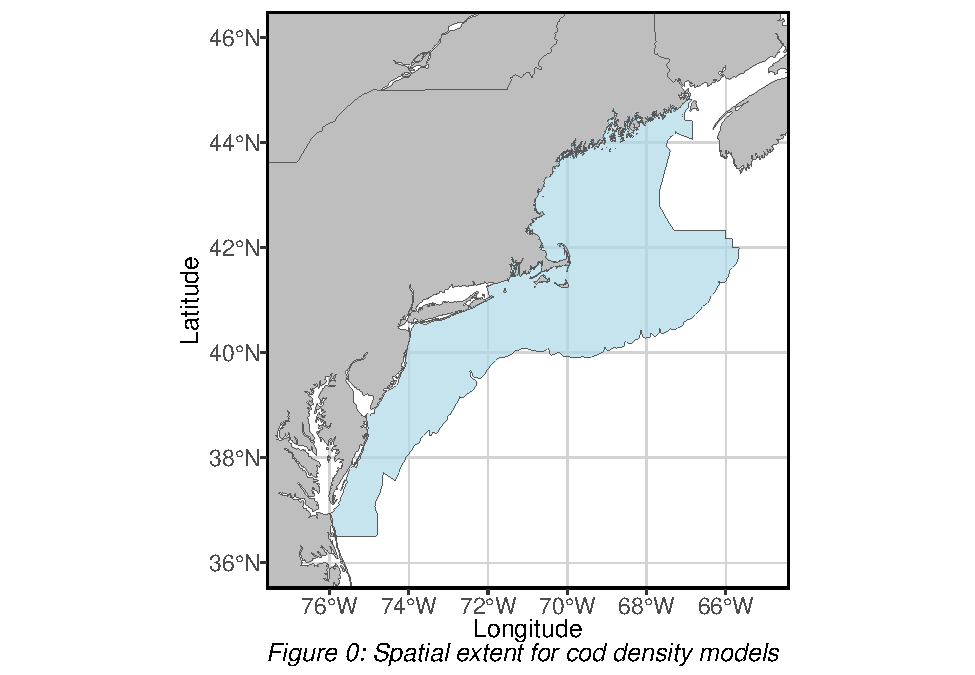
\includegraphics{ToR1_TechPaper_files/figure-latex/total spatial extent-1.pdf}

\hypertarget{vast-spatial-referencing}{%
\subsubsection{VAST spatial referencing}\label{vast-spatial-referencing}}

It has been said that selection of the number of knots and spatial smoothers in VAST is ``an art.'' For now, 200 knot locations will be used to make the SPDE grid on which VAST is run. Knot locations are determined by k-means clustering of the data, and are meant to represent standardized locations optimally placed among all surveyed locations. The model then creates an extrapolation grid. This grid is built on an SPDE approximation to a Matérn correlation function. For this model, anisotropy was expected and therefore included, though its inclusion was assessed in the model selection process. The default number of grid cells (2000) was used in the model, which results in cells that are approximately 25km by 25km.

\begin{figure}
\centering
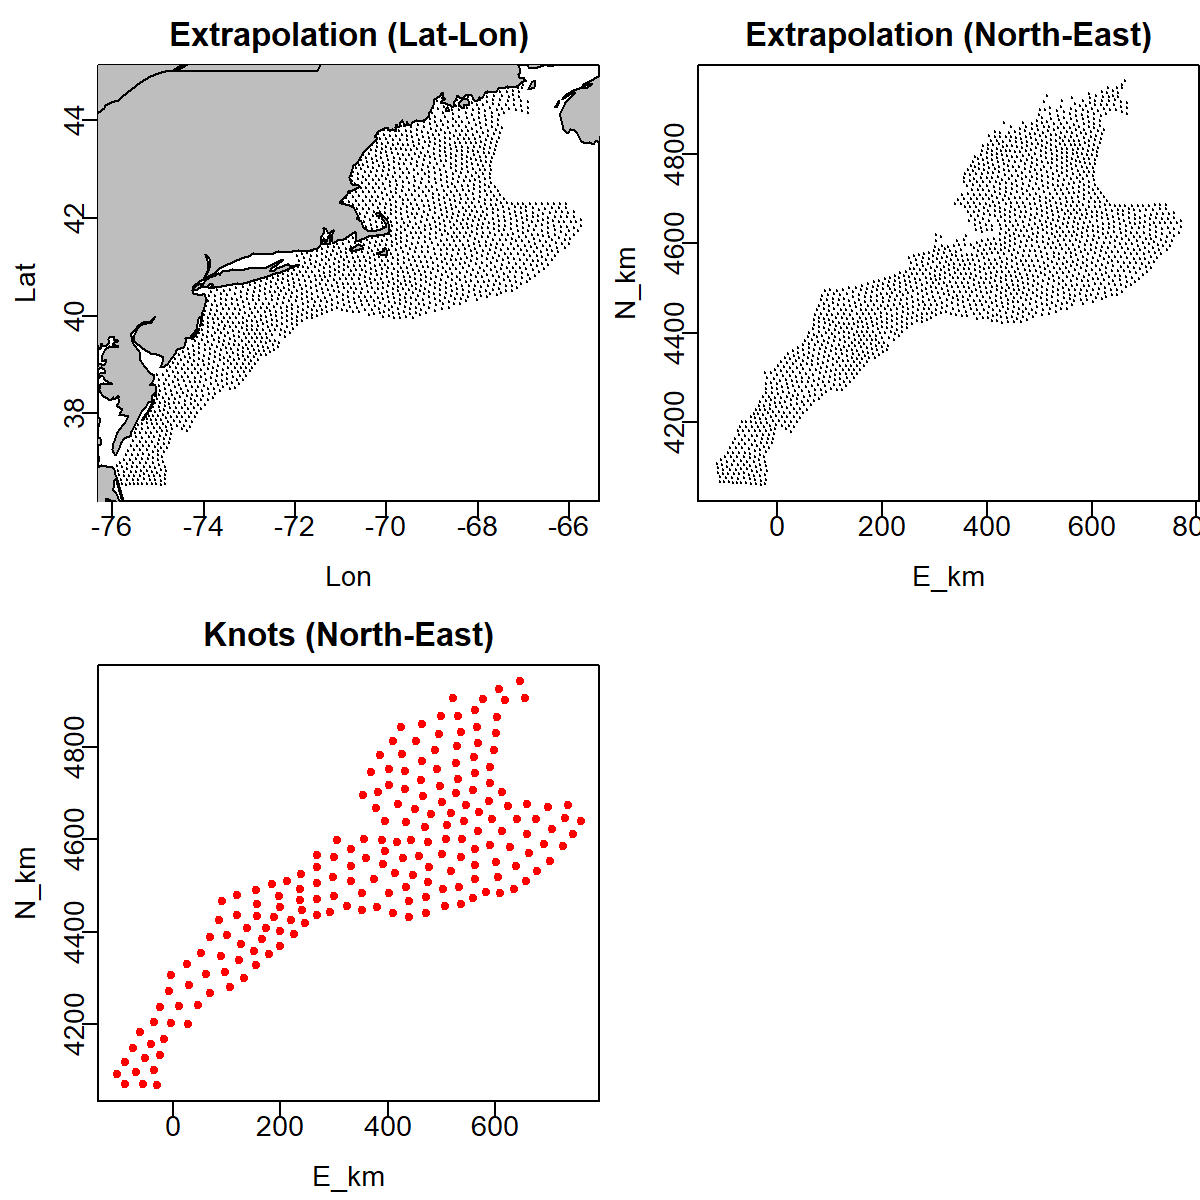
\includegraphics{C:/Users/klankowicz/Documents/GitHub/Atlantic-cod-habitat-VAST/VAST_runs/add_climate_aja4/GBK/Data_and_knots.png}
\caption{Figure 1: Location of extrapolation points and knots within the model spatial domain}
\end{figure}

\hypertarget{strata}{%
\subsubsection{Strata}\label{strata}}

There is evidence that cod spatial density varies among what are known to be distinct cod stock spatial areas (\protect\hyperlink{ref-linner_2022}{Linner and Chen 2022}). The model will therefore be run with each stock area as separate spatial strata (Fig. 2). Metrics of spatial dynamics, indices of abundance, and habitat associations can later be described for each stock area.

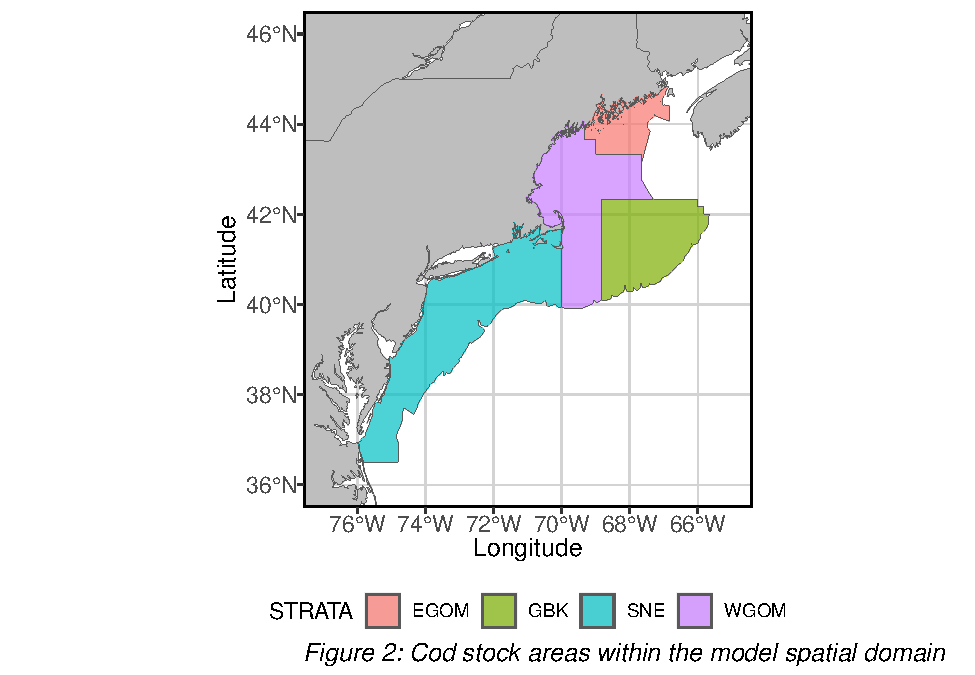
\includegraphics{ToR1_TechPaper_files/figure-latex/spatial strata-1.pdf}

\hypertarget{temporal-extent}{%
\subsubsection{Temporal extent}\label{temporal-extent}}

Though some surveys were initiated in the 1950s and 60s, the time period of interest to this study begins in 1982. Some studies have provided full data from 2022, and others have not. For this reason, the modeled time period will be 1982 - 2021.

\hypertarget{seasonality}{%
\subsubsection{Seasonality}\label{seasonality}}

Time steps in the model will represent the spring and fall seasons of each year in the time series. Therefore, though there are 40 years of data there will be 80 time steps. This distinction is made to capture the seasonal spawning movements of adult cod. The spring season will be March through August of any year \(x\). Fall will be September through December of year \(x\) and January and February of year \(x+1\). This is to ensure that the fall season is temporally continuous, rather than interrupted by the defined spring period.
\#\#\# Categories
Cod were modeled as three separate size classes, as it was expected that habitat utilization and spatial density would vary among size/ age groups. Small fish were defined as shorter than 39.1 cm total length or less than 0.58 kg. Medium fish were between 39.1 and 70.2 cm, or between 0.58 and 3.44 kg. Large fish were longer than 70.2 cm or heavier than 3.44 kg. This size structure roughly matches to ages 0-2 (pre-spawning), ages 2-5 (spawning), and ages 5+ (mature) cod, though this age structure was determined across all years and all spatial areas of the model domains and may be slightly different among time periods and locations. Uncommonly, fish without biological information could still be sorted into size categories. This typically occurred when the total weight of all fish caught in a tow was less than the maximum size limit of a singular small fish-- in this instance, all fish were assumed to belong in the small size category. Fish unable to be assigned to a size category could not be used in the model.

\hypertarget{data-type-link-functions-and-distributions}{%
\subsubsection{Data type, link functions, and distributions}\label{data-type-link-functions-and-distributions}}

VAST models can use biomass, abundance, or encounter data as the response variable to quantify presence at each sampling location. In this model, abundance data were used; not every survey provided biological data including length and weight for every fish sampled, and therefore not every fish could be sorted into a size category by weight as would be necessary for a biomass-data model. As recommended by model developers for abundance-data models, a lognormal-Poisson distribution was chosen for the first linear predictor and an alternative ``Poisson-link delta-model''was chosen for the second linear predictor.

\hypertarget{area-swept}{%
\subsubsection{Area swept}\label{area-swept}}

VAST requires an input for the area swept for each tow. For surveys using bottom trawl methods, area swept was calculated as the distance covered by the tow multiplied by the wing spread. It is recommended that area swept be set to 1 for sampling gears with an unknown effective area swept. Initially, area swept for the bottom longline and Sentinel jigging surveys was set to 1. However, this created an issue of scaling and mixed units. Simple leave-one-out sensitivity tests were run to determine the influence of the bottom longline and Sentinel jigging surveys on the overall cod indices of abundance. Removing the Sentinel jigging survey had little impact on the modeled abundance of all three size classes of cod, and so it was excluded from further analysis. Removing the bottom longline survey reduced the abundance of medium and large cod by up to 50\% in some years, and was therefore retained in further analyses. The description of the bottom longline motivation and methods in McElroy et al. (\protect\hyperlink{ref-mcelroy_2019}{2019}) states that it was developed to as closely as possible match the sampling effort of the NEFSC bottom trawl survey. For this reason, average area swept of the NEFSC bottom trawl survey was also used as the input for the area swept of the bottom longline survey.

\begin{figure}
\centering
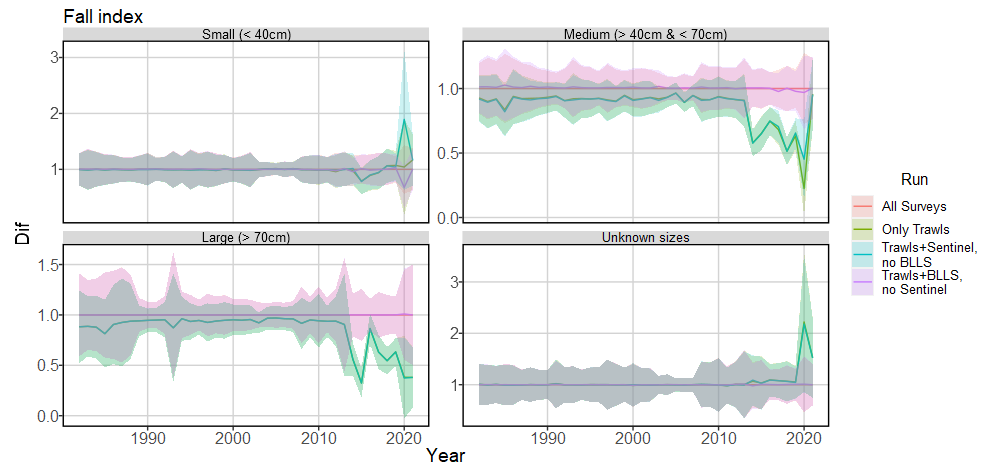
\includegraphics{C:/Users/klankowicz/Documents/GitHub/Atlantic-cod-habitat-VAST/Plot_output/fall_index_proportion_geardrop.png}
\caption{Figure 3: Proportional comparison of fall cod abundance by age group, using model runs with all available data as the control.}
\end{figure}

\begin{figure}
\centering
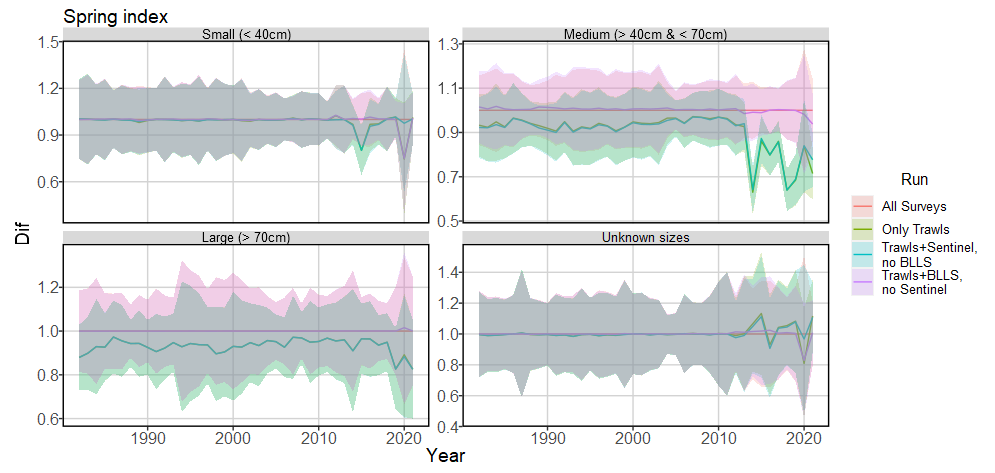
\includegraphics{C:/Users/klankowicz/Documents/GitHub/Atlantic-cod-habitat-VAST/Plot_output/spring_index_proportion_geardrop.png}
\caption{Figure 4: Proportional comparison of spring cod abundance by age group, using model runs with all available data as the control.}
\end{figure}

\hypertarget{vessel-effects}{%
\subsubsection{Vessel effects}\label{vessel-effects}}

Each survey used in this modeling effort has its own set of sampling protocols. It is highly likely that this variability also causes variability in catchability. This random variation in catchability among levels of a grouping variable is referred to as vessel effects in the VAST model structure. For this model, vessel effects were included. It is understood that multiple vessels were sometimes used to complete each survey, but some surveys did not specify the vessel used for each sampling event. Therefore, we simply used survey as the grouping variable rather than vessel. VAST models covariation in vessel effects with a factor model, where variation in catchability between groups is a random effect.

\hypertarget{density-covariates}{%
\subsubsection{Density Covariates}\label{density-covariates}}

VAST allows for the effects of both density and catchability covariates to be included in modeling efforts. Catchability covariates are processes one would expect to affect the ability to observe the target organism without necessarily affecting the distribution of the organism. Density covariates are processes that directly affect the distribution of the target organism, regardless of ability to observe it. Both covariates affect the catch rate of the target organism, but only density covariates are used to predict target organism density within the spatial domain. Therefore, VAST ``controls for'' catchability covariates and ``conditions on'' density covariates. VAST is unable to distinguish whether potential covariates should be treated as catchability or density covariates; this must be decided with theoretical insight from an analyst.

In this model, catchability covariates were not used. As mentioned previously, differences in sampling design were included as vessel effects.

The model will include the effects of several potential density covariates. The final model will only include density covariates with significant impact, as determined by a model selection process that will be discussed later in this document.

\hypertarget{sediment-data}{%
\paragraph{Sediment data}\label{sediment-data}}

Probability of mud, sand, gravel, cobble, and rock substrate existing in 1km by 1km grid cells through the entire continental shelf was provided by Brad Harris and Felipe Restrepo at Alaska Pacific University. These data are a expansion on the New England Fishery Management Council Swept Area Seabed Impact (SASI) model, which previously provided irregular polygons of distinct sediment grain types within the same spatial extent. Sediment observations from historical USGS sediment grabs and UMass Dartmouth's School for Marine Science and Technology (SMAST) video survey program are interpolated using an ordinary kriging approach to create the final 1km by 1km grid of sediment type probability.

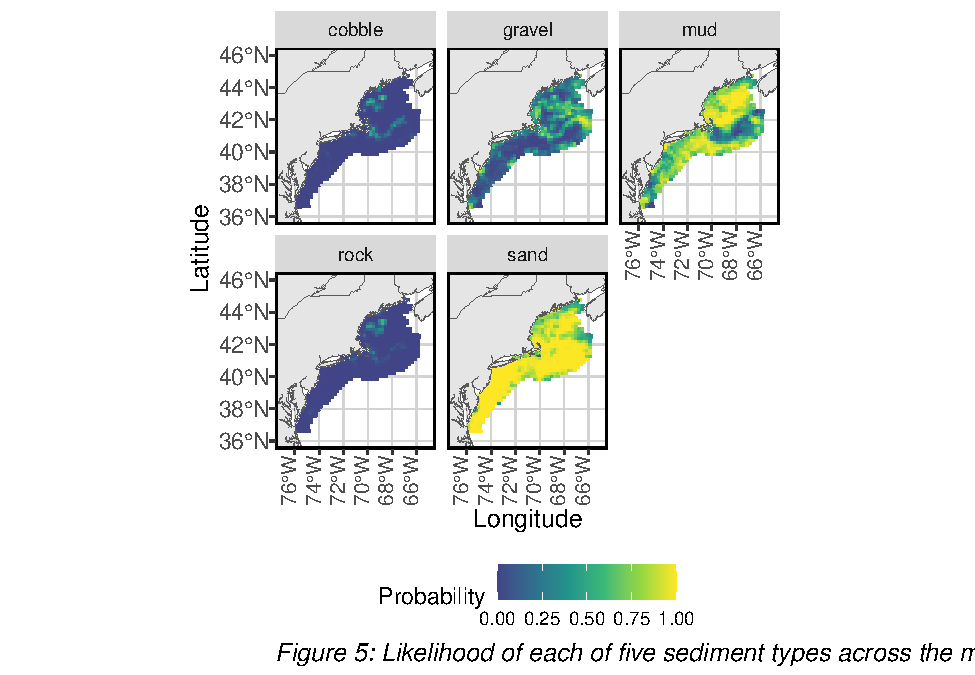
\includegraphics{ToR1_TechPaper_files/figure-latex/sediment plots-1.pdf}

\hypertarget{rugosity}{%
\paragraph{Rugosity}\label{rugosity}}

Rugosity data comes from a dataset created by Ariell Friedman (\protect\hyperlink{ref-friedman_2012}{Friedman et al. 2012}). Rugosity is a unitless measure of elevation change over horizontal distance, and is calculated for grid cells with a 15 arc-second resolution.

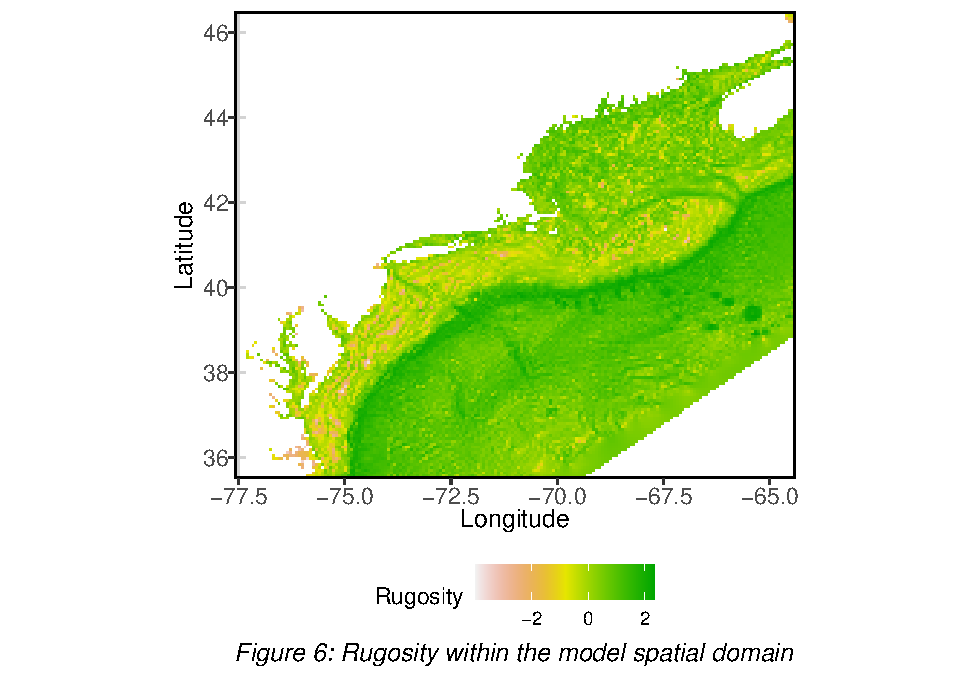
\includegraphics{ToR1_TechPaper_files/figure-latex/rugosity-1.pdf}

\hypertarget{bathymetry}{%
\paragraph{Bathymetry}\label{bathymetry}}

Most surveys recorded average depth at which the various gears were deployed. Some surveys did not provide information regarding gear depth. VAST models cannot have missing values in the density covariate inputs, so this inconsistency was an issue. Therefore, instead of using survey-reported values, depth at all survey locations was interpolated from GEBCO 15 arc-second bathymetry.

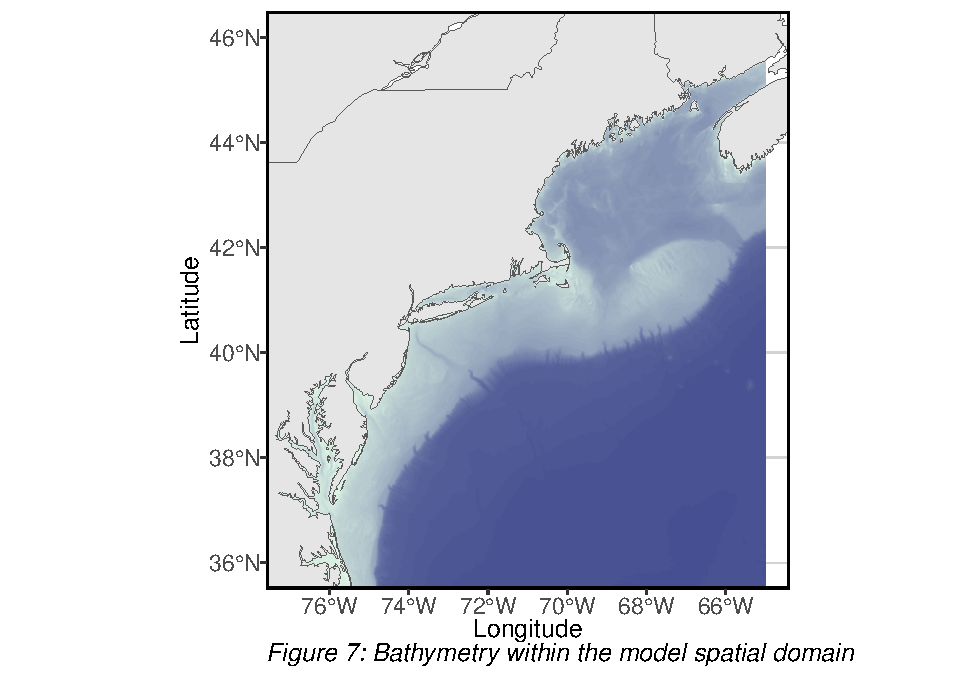
\includegraphics{ToR1_TechPaper_files/figure-latex/bathy-1.pdf}

\hypertarget{sea-surface-temperature}{%
\paragraph{Sea Surface Temperature}\label{sea-surface-temperature}}

The previous density covariates were temporally stationary. The following measures of temperature are temporally dynamic. For sea surface temperature, OISST values were pulled from NOAA data sources and extracted at observation locations. OISST values were compared to field measurements, when available, and the two were found to be generally similar. The following plot describes overall differences between field-measured SST and OISST when both measures were available for the same observation.

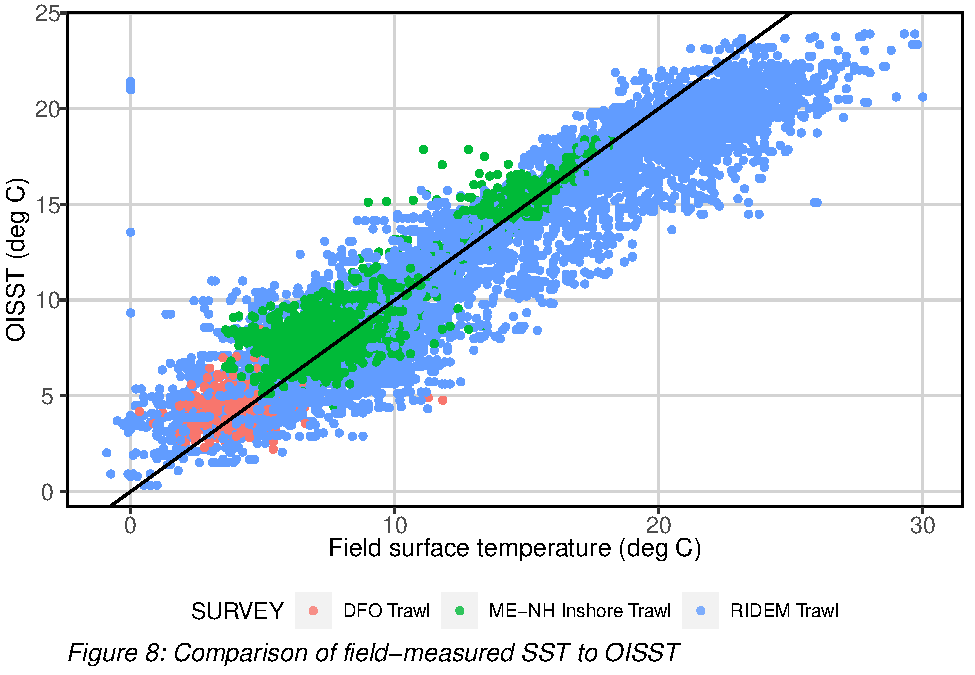
\includegraphics{ToR1_TechPaper_files/figure-latex/oisst-1.pdf}

\hypertarget{bottom-temperature}{%
\paragraph{Bottom Temperature}\label{bottom-temperature}}

Bottom temperature data were provided by Du Pontavice et al. (\protect\hyperlink{ref-du_pontavice_2023}{2023}). Bottom temperature within approximately 5' by 5' grid cells were calculated at a daily timestep for 1982 to 2020. Because cod observation data were collected through 2021, bottom temperature data for this year were simply copied from 2020. This may not be accurate, and it may be better to exclude 2021 data in future efforts. Further, the bottom temperature product did not extend to the inshore strata included in the model. To fix this issue, bottom temperature was interpolated to the inshore strata from the existing data.

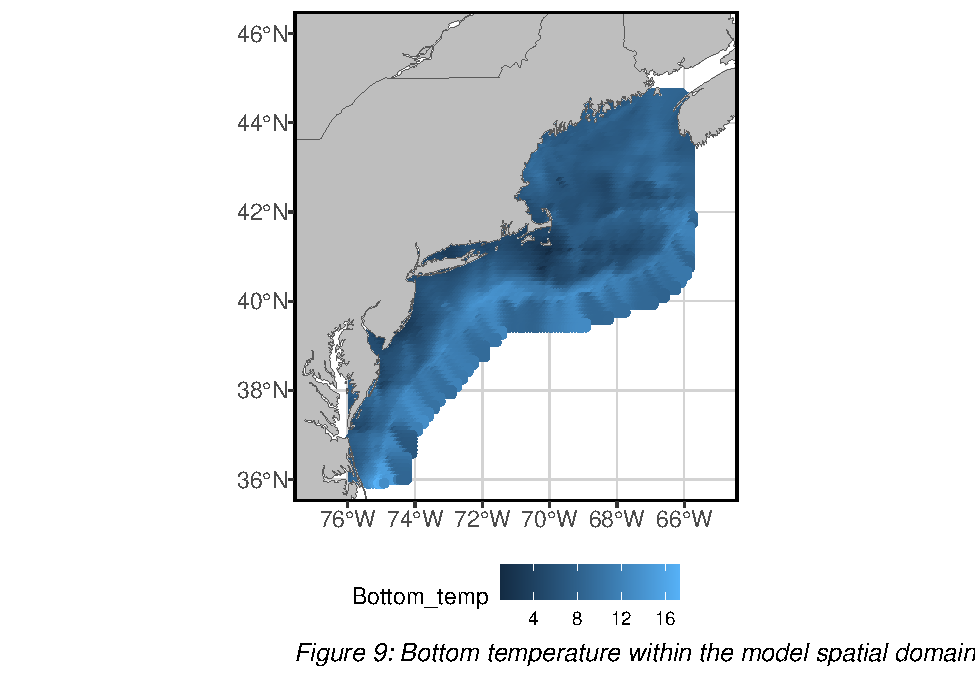
\includegraphics{ToR1_TechPaper_files/figure-latex/bottom temp-1.pdf}

\hypertarget{climate-indices}{%
\paragraph{Climate Indices}\label{climate-indices}}

Several climate indices have been demonstrated to have a relationship to cod abundance and distribution. For this model, NAO and AMO data were used as climate indices and tested for inclusion in the final model. NAO data are provided at a daily timestep within the model, whereas AMO was provided at a monthly timestep. Both were basin-wide indices, meaning the value does not change between spatial locations within the region.

\hypertarget{density-covariate-collinearity}{%
\subsubsection{Density Covariate Collinearity}\label{density-covariate-collinearity}}

Potential density covariates were tested for collinearity. High correlations were found between two pairs: cobble and rock probability within 1km grid cells, and OISST and bottom temperature. Probability of rock and OISST were removed as covariates. For the first pair, rock was removed as bottom sample grabs (the bulk of sediment samples that make up the dataset) are more likely able to accurately characterize cobble distribution than larger boulders. For the second pair, OISST was removed as cod are groundfish and therefore more likely to be affected by bottom temperature than surface temperature. Once these two collinear relationships were addressed, the remainder of density covariates were not correlated and therefore were included in the model.

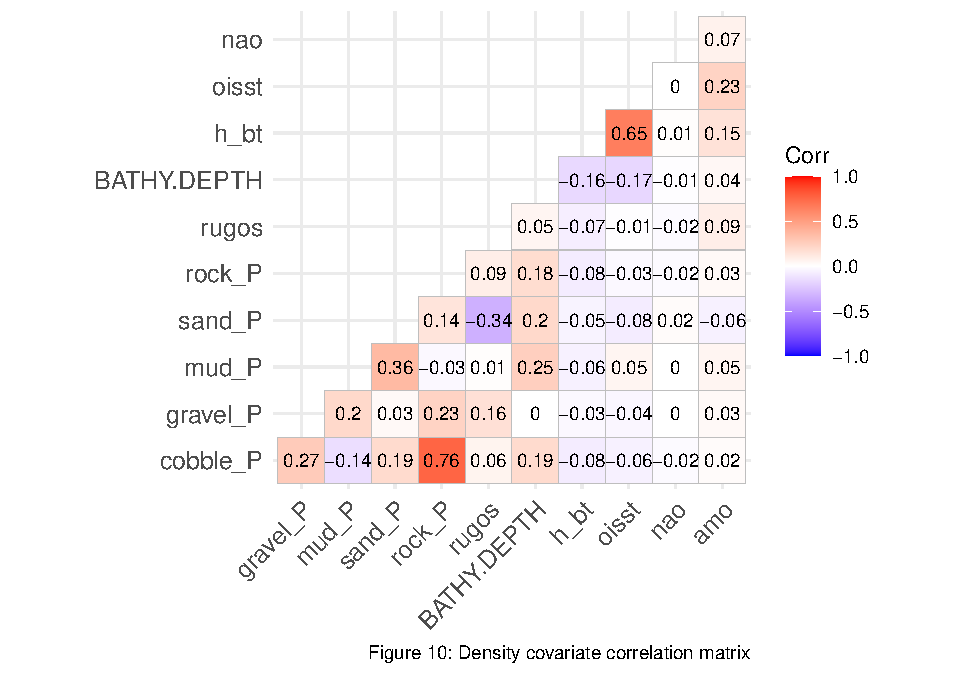
\includegraphics{ToR1_TechPaper_files/figure-latex/collinearity-1.pdf}

\hypertarget{model-selection}{%
\subsection{Model selection}\label{model-selection}}

The model selection process was completed in two steps. The first step compared models with and without anisotropy and/ or spatial and spatiotemporal random effects in the first and second linear predictors. This follows the model selection process of Ng et al. (\protect\hyperlink{ref-ng_2021}{2021}). The second step was to compare models with all possible combinations of the nine density covariates

\hypertarget{model-settings-selection}{%
\subsubsection{Model settings selection}\label{model-settings-selection}}

Model settings were explored using model selection. Models were tested for different values in the Field Configuration settings (testing the use of spatial and spatiotemporal variation in the linear predictors), anisotropy, and overdispersion. AIC was used to compare models and restricted maximum likelihood (REML) was used in model construction to make comparison via AIC possible (\protect\hyperlink{ref-zuur_2009}{Zuur et al. 2009}).

Model naming conventions are as follows:

\begin{itemize}
\tightlist
\item
  ``alleffectson'' - anisotropy on, spatial and spatiotemporal random effects in both linear predictors
\item
  ``noaniso'' - anisotropy off, spatial and spatiotemporal random effects in both linear predictors
\item
  ``noomeps2'' - anisotropy and spatial and spatiotemporal effects in linear predictor 1
\item
  ``noomeps2\_noaniso'' - anisotropy off, spatial and spatiotemporal effects in linear predictor 1
\item
  ``noomeps2\_noeps1'' - anisotropy and spatial effects in linear predictor 1
\item
  ``noomeps2\_noeps1\_noaniso'' - anisotropy off, spatial effects in linear predictor 1
\item
  ``noomeps12'' - anisotropy on, no spatial or spatiotemporal effects
\item
  ``noomeps12\_noaniso'' - anisotropy off, no spatial or spatiotemporal effects
\end{itemize}

The best model included anisotropy and spatial and spatiotemporal effects in both linear predictors.

\begin{table}[H]

\caption{(\#tab:settings selection)Table 1: Model selection step 1 outcomes}
\centering
\begin{tabular}[t]{lrrrrl}
\toprule
Model name & delta AIC & Fixed coefficients & Random coefficients & AIC & converged\\
\midrule
\cellcolor{gray!10}{alleffectson} & \cellcolor{gray!10}{0.000000e+00} & \cellcolor{gray!10}{9} & \cellcolor{gray!10}{41790} & \cellcolor{gray!10}{60128.32} & \cellcolor{gray!10}{likely}\\
noaniso & 2.407274e-01 & 7 & 41790 & 60128.56 & likely\\
\cellcolor{gray!10}{noomeps2\_noaniso} & \cellcolor{gray!10}{1.720459e+03} & \cellcolor{gray!10}{4} & \cellcolor{gray!10}{20973} & \cellcolor{gray!10}{61848.78} & \cellcolor{gray!10}{likely}\\
noomeps2 & 1.720765e+03 & 6 & 20973 & 61849.08 & likely\\
\cellcolor{gray!10}{noomeps2\_noeps1} & \cellcolor{gray!10}{3.448233e+03} & \cellcolor{gray!10}{5} & \cellcolor{gray!10}{413} & \cellcolor{gray!10}{63576.55} & \cellcolor{gray!10}{likely}\\
\addlinespace
noomeps2\_noeps1\_noaniso & 3.451895e+03 & 3 & 413 & 63580.21 & likely\\
\cellcolor{gray!10}{noomeps12} & \cellcolor{gray!10}{1.283181e+04} & \cellcolor{gray!10}{1} & \cellcolor{gray!10}{156} & \cellcolor{gray!10}{72960.13} & \cellcolor{gray!10}{likely}\\
noomeps12\_noaniso & 1.283181e+04 & 1 & 156 & 72960.13 & likely\\
\bottomrule
\end{tabular}
\end{table}

\hypertarget{density-covariate-selection}{%
\subsubsection{Density covariate selection}\label{density-covariate-selection}}

Density covariates were selected for inclusion into the final model by running a subset of the original observation data (last 5 years of NEFSC bottom trawl data) with all possible combinations of variables as spatial density inputs. The four sediment likelihood variables (cobble, gravel, sand, and mud) were never separated. Models were then compared using AIC. Maximum likelihood was used to calculate AIC, as the spatial and spatiotemporal random effects did not change between models.

Model naming conventions are as follows:

\begin{itemize}
\tightlist
\item
  ``seds'' - all sediment likeihood variables (cobble, gravel, sand, and mud)
\item
  ``rugos'' - rugosity
\item
  ``bathy'' - bathymetry
\item
  ``bottom'' - bottom temperature
\item
  ``nao'' - daily North Atlantic Oscillation index
\item
  ``amo'' - monthly North Atlantic Oscillation index
\end{itemize}

The model with the lowest AIC was the model that included spatial density terms for all potential covariates.

\begin{table}[H]

\caption{\label{tab:covars}Table 2a: Model selection step 2 outcomes}
\centering
\begin{tabular}[t]{lrrrr}
\toprule
Model name & delta AIC & Fixed coefficients & Random coefficients & AIC\\
\midrule
\cellcolor{gray!10}{sedsrugosbathybottomnaoamo} & \cellcolor{gray!10}{0.0000000} & \cellcolor{gray!10}{47} & \cellcolor{gray!10}{5632} & \cellcolor{gray!10}{31827.73}\\
sedsrugosbathybottomamo & 0.2068173 & 45 & 5632 & 31827.94\\
\cellcolor{gray!10}{sedsrugosbathybottomnao} & \cellcolor{gray!10}{0.7153067} & \cellcolor{gray!10}{45} & \cellcolor{gray!10}{5632} & \cellcolor{gray!10}{31828.44}\\
sedsrugosbathybottom & 1.4555360 & 43 & 5632 & 31829.18\\
\cellcolor{gray!10}{sedsrugosbathynaoamo} & \cellcolor{gray!10}{24.2643819} & \cellcolor{gray!10}{45} & \cellcolor{gray!10}{5632} & \cellcolor{gray!10}{31851.99}\\
\addlinespace
sedsrugosbathyamo & 24.6986828 & 43 & 5632 & 31852.43\\
\cellcolor{gray!10}{sedsbathybottomnaoamo} & \cellcolor{gray!10}{29.2902682} & \cellcolor{gray!10}{45} & \cellcolor{gray!10}{5632} & \cellcolor{gray!10}{31857.02}\\
sedsbathybottomamo & 29.6062683 & 43 & 5632 & 31857.34\\
\cellcolor{gray!10}{sedsbathybottomnao} & \cellcolor{gray!10}{30.1573439} & \cellcolor{gray!10}{43} & \cellcolor{gray!10}{5632} & \cellcolor{gray!10}{31857.89}\\
sedsrugosbathynao & 30.4622757 & 43 & 5632 & 31858.19\\
\addlinespace
\cellcolor{gray!10}{sedsbathybottom} & \cellcolor{gray!10}{31.0567709} & \cellcolor{gray!10}{41} & \cellcolor{gray!10}{5632} & \cellcolor{gray!10}{31858.79}\\
sedsrugosbathy & 31.8155721 & 41 & 5632 & 31859.54\\
\cellcolor{gray!10}{sedsbathynaoamo} & \cellcolor{gray!10}{52.4577598} & \cellcolor{gray!10}{43} & \cellcolor{gray!10}{5632} & \cellcolor{gray!10}{31880.19}\\
sedsbathyamo & 53.0261733 & 41 & 5632 & 31880.76\\
\cellcolor{gray!10}{sedsbathynao} & \cellcolor{gray!10}{58.7423222} & \cellcolor{gray!10}{41} & \cellcolor{gray!10}{5632} & \cellcolor{gray!10}{31886.47}\\
\addlinespace
sedsbathy & 60.2936041 & 39 & 5632 & 31888.02\\
\cellcolor{gray!10}{rugosbathybottomamo} & \cellcolor{gray!10}{62.3041648} & \cellcolor{gray!10}{37} & \cellcolor{gray!10}{5632} & \cellcolor{gray!10}{31890.03}\\
rugosbathybottomnaoamo & 63.0030174 & 39 & 5632 & 31890.73\\
\cellcolor{gray!10}{rugosbathybottom} & \cellcolor{gray!10}{63.9483351} & \cellcolor{gray!10}{35} & \cellcolor{gray!10}{5632} & \cellcolor{gray!10}{31891.68}\\
rugosbathybottomnao & 64.1454668 & 37 & 5632 & 31891.87\\
\addlinespace
\cellcolor{gray!10}{bathybottomamo} & \cellcolor{gray!10}{84.2510758} & \cellcolor{gray!10}{35} & \cellcolor{gray!10}{5632} & \cellcolor{gray!10}{31911.98}\\
bathybottomnaoamo & 84.7596911 & 37 & 5632 & 31912.49\\
\cellcolor{gray!10}{rugosbathyamo} & \cellcolor{gray!10}{85.4995550} & \cellcolor{gray!10}{35} & \cellcolor{gray!10}{5632} & \cellcolor{gray!10}{31913.23}\\
rugosbathynaoamo & 85.9832816 & 37 & 5632 & 31913.71\\
\cellcolor{gray!10}{bathybottomnao} & \cellcolor{gray!10}{86.0862582} & \cellcolor{gray!10}{35} & \cellcolor{gray!10}{5632} & \cellcolor{gray!10}{31913.82}\\
\addlinespace
bathybottom & 86.1266561 & 33 & 5632 & 31913.86\\
\cellcolor{gray!10}{rugosbathynao} & \cellcolor{gray!10}{92.5446440} & \cellcolor{gray!10}{35} & \cellcolor{gray!10}{5632} & \cellcolor{gray!10}{31920.27}\\
rugosbathy & 92.9041665 & 33 & 5632 & 31920.63\\
\cellcolor{gray!10}{bathyamo} & \cellcolor{gray!10}{106.5076105} & \cellcolor{gray!10}{33} & \cellcolor{gray!10}{5632} & \cellcolor{gray!10}{31934.24}\\
bathynaoamo & 106.7738774 & 35 & 5632 & 31934.50\\
\addlinespace
\cellcolor{gray!10}{bathynao} & \cellcolor{gray!10}{113.4711624} & \cellcolor{gray!10}{33} & \cellcolor{gray!10}{5632} & \cellcolor{gray!10}{31941.20}\\
bathy & 114.1115364 & 31 & 5632 & 31941.84\\
\cellcolor{gray!10}{sedsrugosbottomnao} & \cellcolor{gray!10}{249.0554839} & \cellcolor{gray!10}{43} & \cellcolor{gray!10}{5632} & \cellcolor{gray!10}{32076.78}\\
sedsrugosbottomnaoamo & 249.7008586 & 45 & 5632 & 32077.43\\
\cellcolor{gray!10}{sedsrugosbottom} & \cellcolor{gray!10}{250.3797688} & \cellcolor{gray!10}{41} & \cellcolor{gray!10}{5632} & \cellcolor{gray!10}{32078.11}\\
\bottomrule
\end{tabular}
\end{table}

\begin{table}[H]

\caption{\label{tab:covars}Table 2b: Model selection step 2 outcomes}
\centering
\begin{tabular}[t]{lrrrr}
\toprule
Model name & delta AIC & Fixed coefficients & Random coefficients & AIC\\
\midrule
\cellcolor{gray!10}{sedsrugosbottomamo} & \cellcolor{gray!10}{250.5617} & \cellcolor{gray!10}{43} & \cellcolor{gray!10}{5632} & \cellcolor{gray!10}{32078.29}\\
sedsbottomnao & 269.8470 & 41 & 5632 & 32097.58\\
\cellcolor{gray!10}{sedsbottomnaoamo} & \cellcolor{gray!10}{270.2860} & \cellcolor{gray!10}{43} & \cellcolor{gray!10}{5632} & \cellcolor{gray!10}{32098.01}\\
sedsbottomamo & 271.1444 & 41 & 5632 & 32098.87\\
\cellcolor{gray!10}{sedsbottom} & \cellcolor{gray!10}{271.2075} & \cellcolor{gray!10}{39} & \cellcolor{gray!10}{5632} & \cellcolor{gray!10}{32098.94}\\
\addlinespace
sedsrugosnaoamo & 295.7166 & 43 & 5632 & 32123.45\\
\cellcolor{gray!10}{sedsrugosamo} & \cellcolor{gray!10}{297.0664} & \cellcolor{gray!10}{41} & \cellcolor{gray!10}{5632} & \cellcolor{gray!10}{32124.80}\\
sedsrugosnao & 301.6872 & 41 & 5632 & 32129.42\\
\cellcolor{gray!10}{sedsrugos} & \cellcolor{gray!10}{304.0014} & \cellcolor{gray!10}{39} & \cellcolor{gray!10}{5632} & \cellcolor{gray!10}{32131.73}\\
sedsnaoamo & 314.6790 & 41 & 5632 & 32142.41\\
\addlinespace
\cellcolor{gray!10}{sedsamo} & \cellcolor{gray!10}{316.0543} & \cellcolor{gray!10}{39} & \cellcolor{gray!10}{5632} & \cellcolor{gray!10}{32143.78}\\
sedsnao & 320.8598 & 39 & 5632 & 32148.59\\
\cellcolor{gray!10}{seds} & \cellcolor{gray!10}{323.2514} & \cellcolor{gray!10}{37} & \cellcolor{gray!10}{5632} & \cellcolor{gray!10}{32150.98}\\
rugosbottom & 406.3812 & 33 & 5632 & 32234.11\\
\cellcolor{gray!10}{rugosbottomnao} & \cellcolor{gray!10}{406.5037} & \cellcolor{gray!10}{35} & \cellcolor{gray!10}{5632} & \cellcolor{gray!10}{32234.23}\\
\addlinespace
rugosbottomamo & 407.0379 & 35 & 5632 & 32234.77\\
\cellcolor{gray!10}{rugosbottomnaoamo} & \cellcolor{gray!10}{407.5113} & \cellcolor{gray!10}{37} & \cellcolor{gray!10}{5632} & \cellcolor{gray!10}{32235.24}\\
bottomnao & 423.8988 & 33 & 5632 & 32251.63\\
\cellcolor{gray!10}{bottom} & \cellcolor{gray!10}{423.9570} & \cellcolor{gray!10}{31} & \cellcolor{gray!10}{5632} & \cellcolor{gray!10}{32251.69}\\
bottomamo & 424.3848 & 33 & 5632 & 32252.11\\
\addlinespace
\cellcolor{gray!10}{bottomnaoamo} & \cellcolor{gray!10}{424.7147} & \cellcolor{gray!10}{35} & \cellcolor{gray!10}{5632} & \cellcolor{gray!10}{32252.44}\\
rugosamo & 460.7255 & 33 & 5632 & 32288.45\\
\cellcolor{gray!10}{rugosnaoamo} & \cellcolor{gray!10}{460.7792} & \cellcolor{gray!10}{35} & \cellcolor{gray!10}{5632} & \cellcolor{gray!10}{32288.51}\\
rugosnao & 466.5960 & 33 & 5632 & 32294.32\\
\cellcolor{gray!10}{rugos} & \cellcolor{gray!10}{467.3466} & \cellcolor{gray!10}{31} & \cellcolor{gray!10}{5632} & \cellcolor{gray!10}{32295.08}\\
\addlinespace
naoamo & 476.5718 & 33 & 5632 & 32304.30\\
\cellcolor{gray!10}{amo} & \cellcolor{gray!10}{476.6922} & \cellcolor{gray!10}{31} & \cellcolor{gray!10}{5632} & \cellcolor{gray!10}{32304.42}\\
nao & 482.6383 & 31 & 5632 & 32310.37\\
\cellcolor{gray!10}{base} & \cellcolor{gray!10}{483.6222} & \cellcolor{gray!10}{29} & \cellcolor{gray!10}{5632} & \cellcolor{gray!10}{32311.35}\\
\bottomrule
\end{tabular}
\end{table}

\hypertarget{final-model}{%
\subsection{Final model}\label{final-model}}

After the model selection process, the best model included anisotropy, spatial, and spatiotemporal random effects in both linear predictors and density covariates for four classes of sediment types, rugosity, bathymetry, bottom temperature, NAO index, and AMO index. The model was structured with 200 knots and a Matern process spatial smoother to create 2000 grid cells of approximately 25km by 25km to extrapolate spatial density of three size classes of Atlantic cod in both the spring and fall seasons of each year from 1982 - 2021. The final model was also run with bias correction turned on, which uses the ``epsilon method'' to ensure that the mean and variation of generated indices of abundance are not biased due to their transformation by a nonlinear function in the modeling process (\protect\hyperlink{ref-thorson_2016}{Thorson and Kristensen 2016}).

\hypertarget{results}{%
\section{Results}\label{results}}

\hypertarget{spring-index}{%
\subsection{Spring Index}\label{spring-index}}

Large cod had the lowest abundance within the study area of all three size classes, and abundance for this group decreased over time. This result held for indices calculated within each of the four stock areas as well. Large cod were most abundant in the Georges Bank stock area. The center of gravity for large cod tended to be within the Georges Bank stock area and shifted slightly offshore over the time series. Effective area occupied decreased dramatically over time.

Medium cod had higher abundance than large cod, but also had a decreasing abundance trend over time. Similar to large cod, this result held when separating indices of abundance into each of the stock areas. Medium cod were most abundant in the Western Gulf of Maine stock area. The center of gravity for medium cod was typically on the border between the Western Gulf of Maine stock area and the Georges Bank stock area, and moved slightly offshore over time. Effective area occupied decreased over time.

Small cod had high variability through the time series, and seemed to have a jump in recruitment at around 2003. There is no clear trend in small cod abundance over time, though there may have been a slight increasing trend since 2003. Small cod are most abundant in the Southern New England stock area. The center of gravity for small cod was typically in either Southern New England or Western Gulf of Maine waters around Cape Cod, though occasional strong abundance years for coastal Maine pulled the center of gravity dramatically northwards. There is no clear trend for changes in effective area occupied over time.

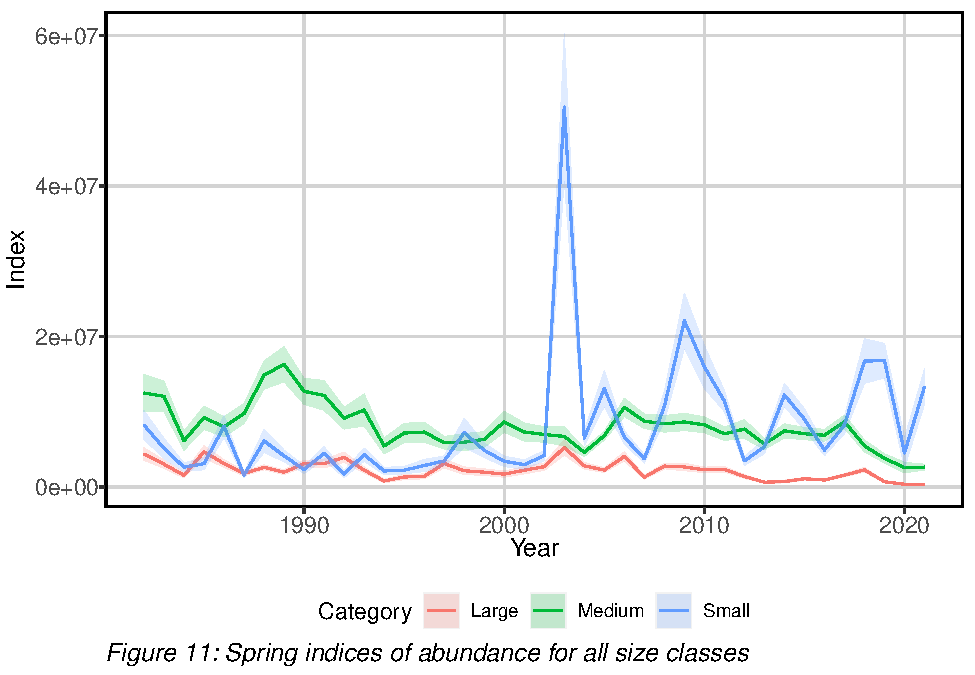
\includegraphics{ToR1_TechPaper_files/figure-latex/spring index-1.pdf} 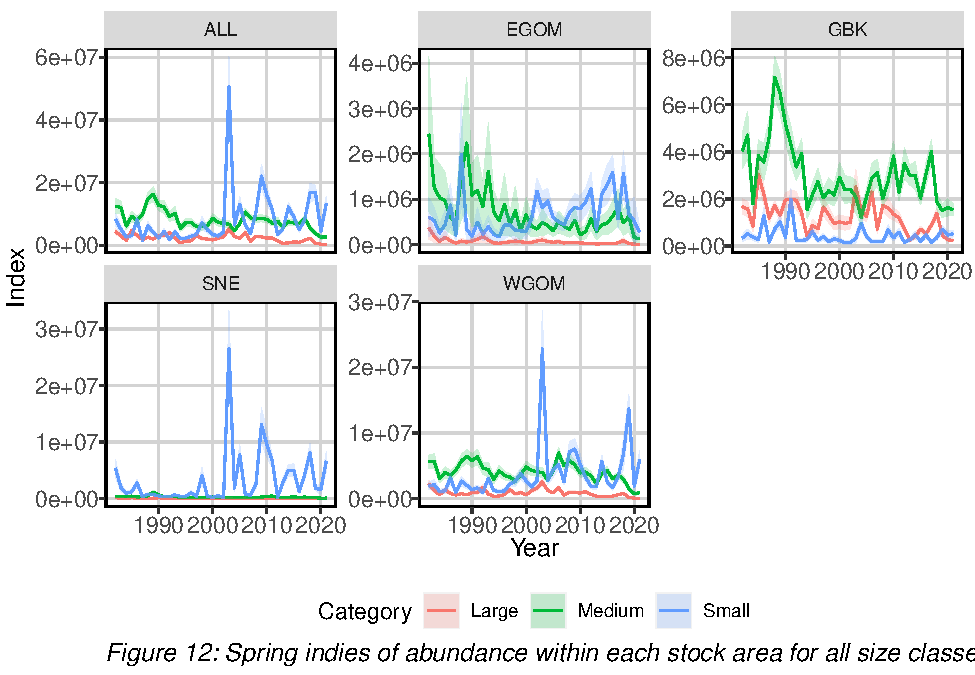
\includegraphics{ToR1_TechPaper_files/figure-latex/spring index-2.pdf}

\begin{figure}
\centering
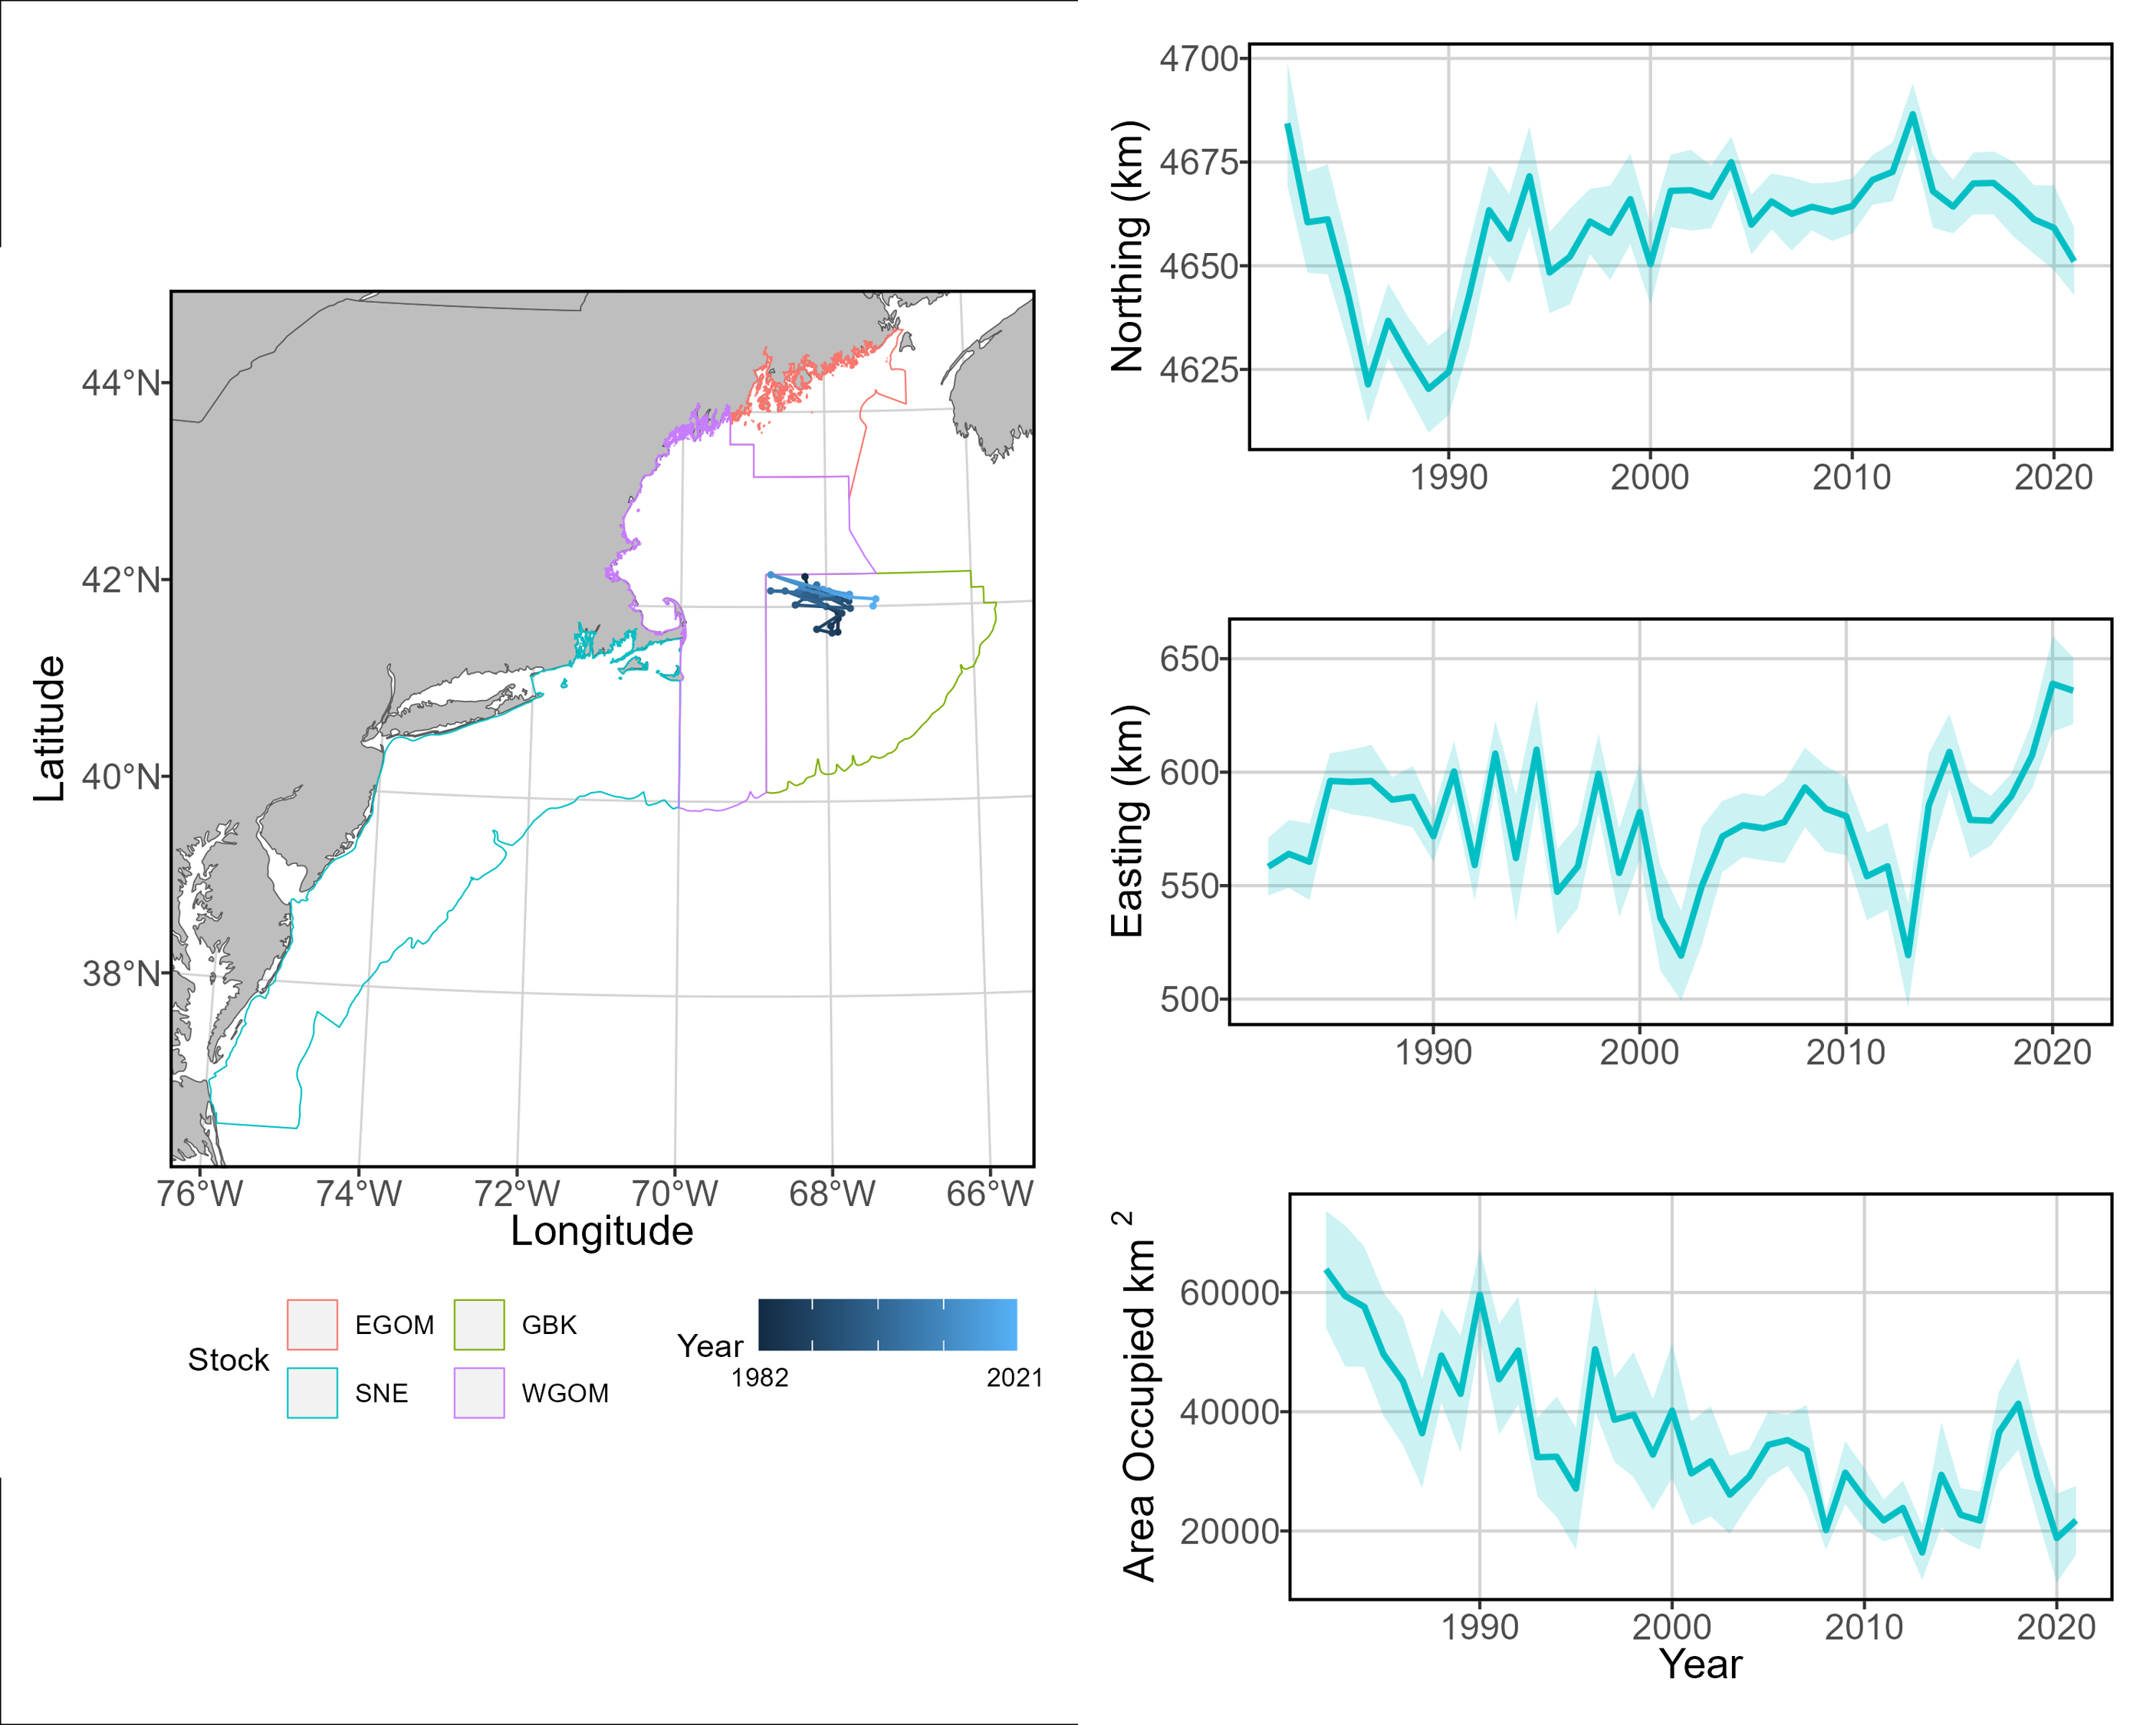
\includegraphics{C:/Users/klankowicz/Documents/GitHub/Atlantic-cod-habitat-VAST/Plot_output_4/large.spring.png}
\caption{Figure 13: Large cod center of gravity and effective area occupied for all stock areas, spring seasons 1982 - 2021.}
\end{figure}

\begin{figure}
\centering
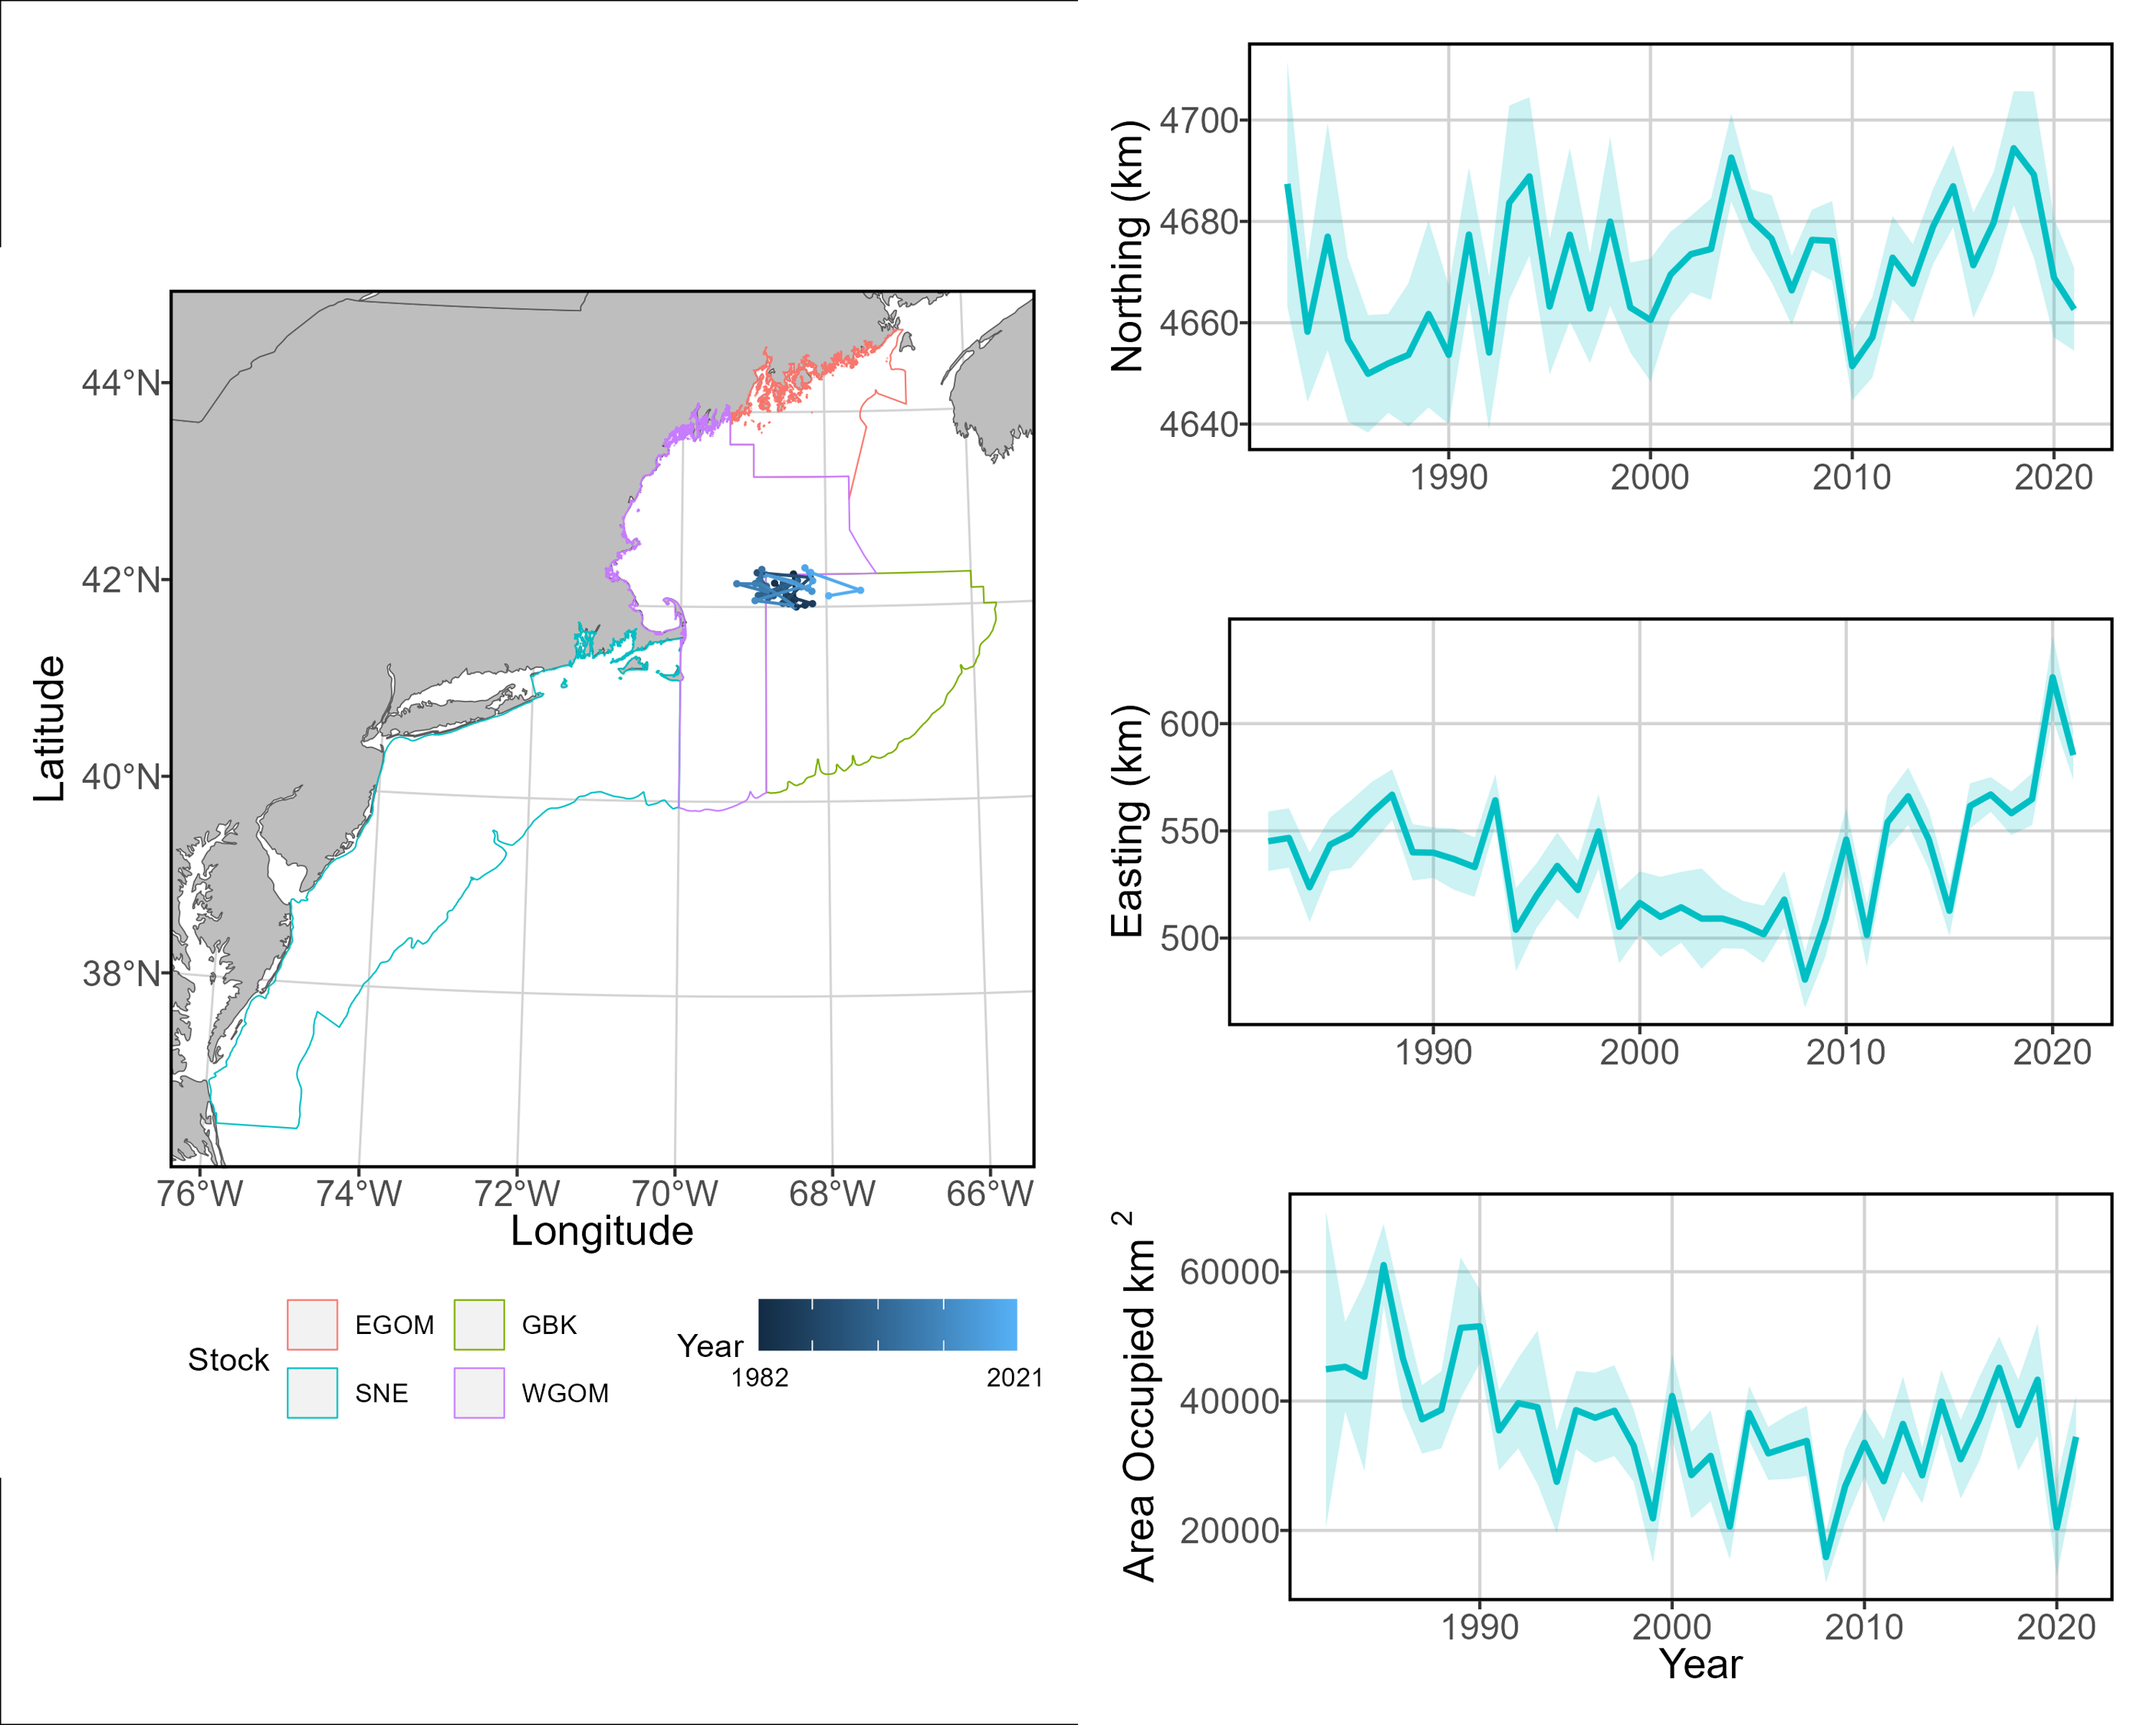
\includegraphics{C:/Users/klankowicz/Documents/GitHub/Atlantic-cod-habitat-VAST/Plot_output_4/medium.spring.png}
\caption{Figure 14: Medium cod center of gravity and effective area occupied for all stock areas, spring seasons 1982 - 2021.}
\end{figure}

\begin{figure}
\centering
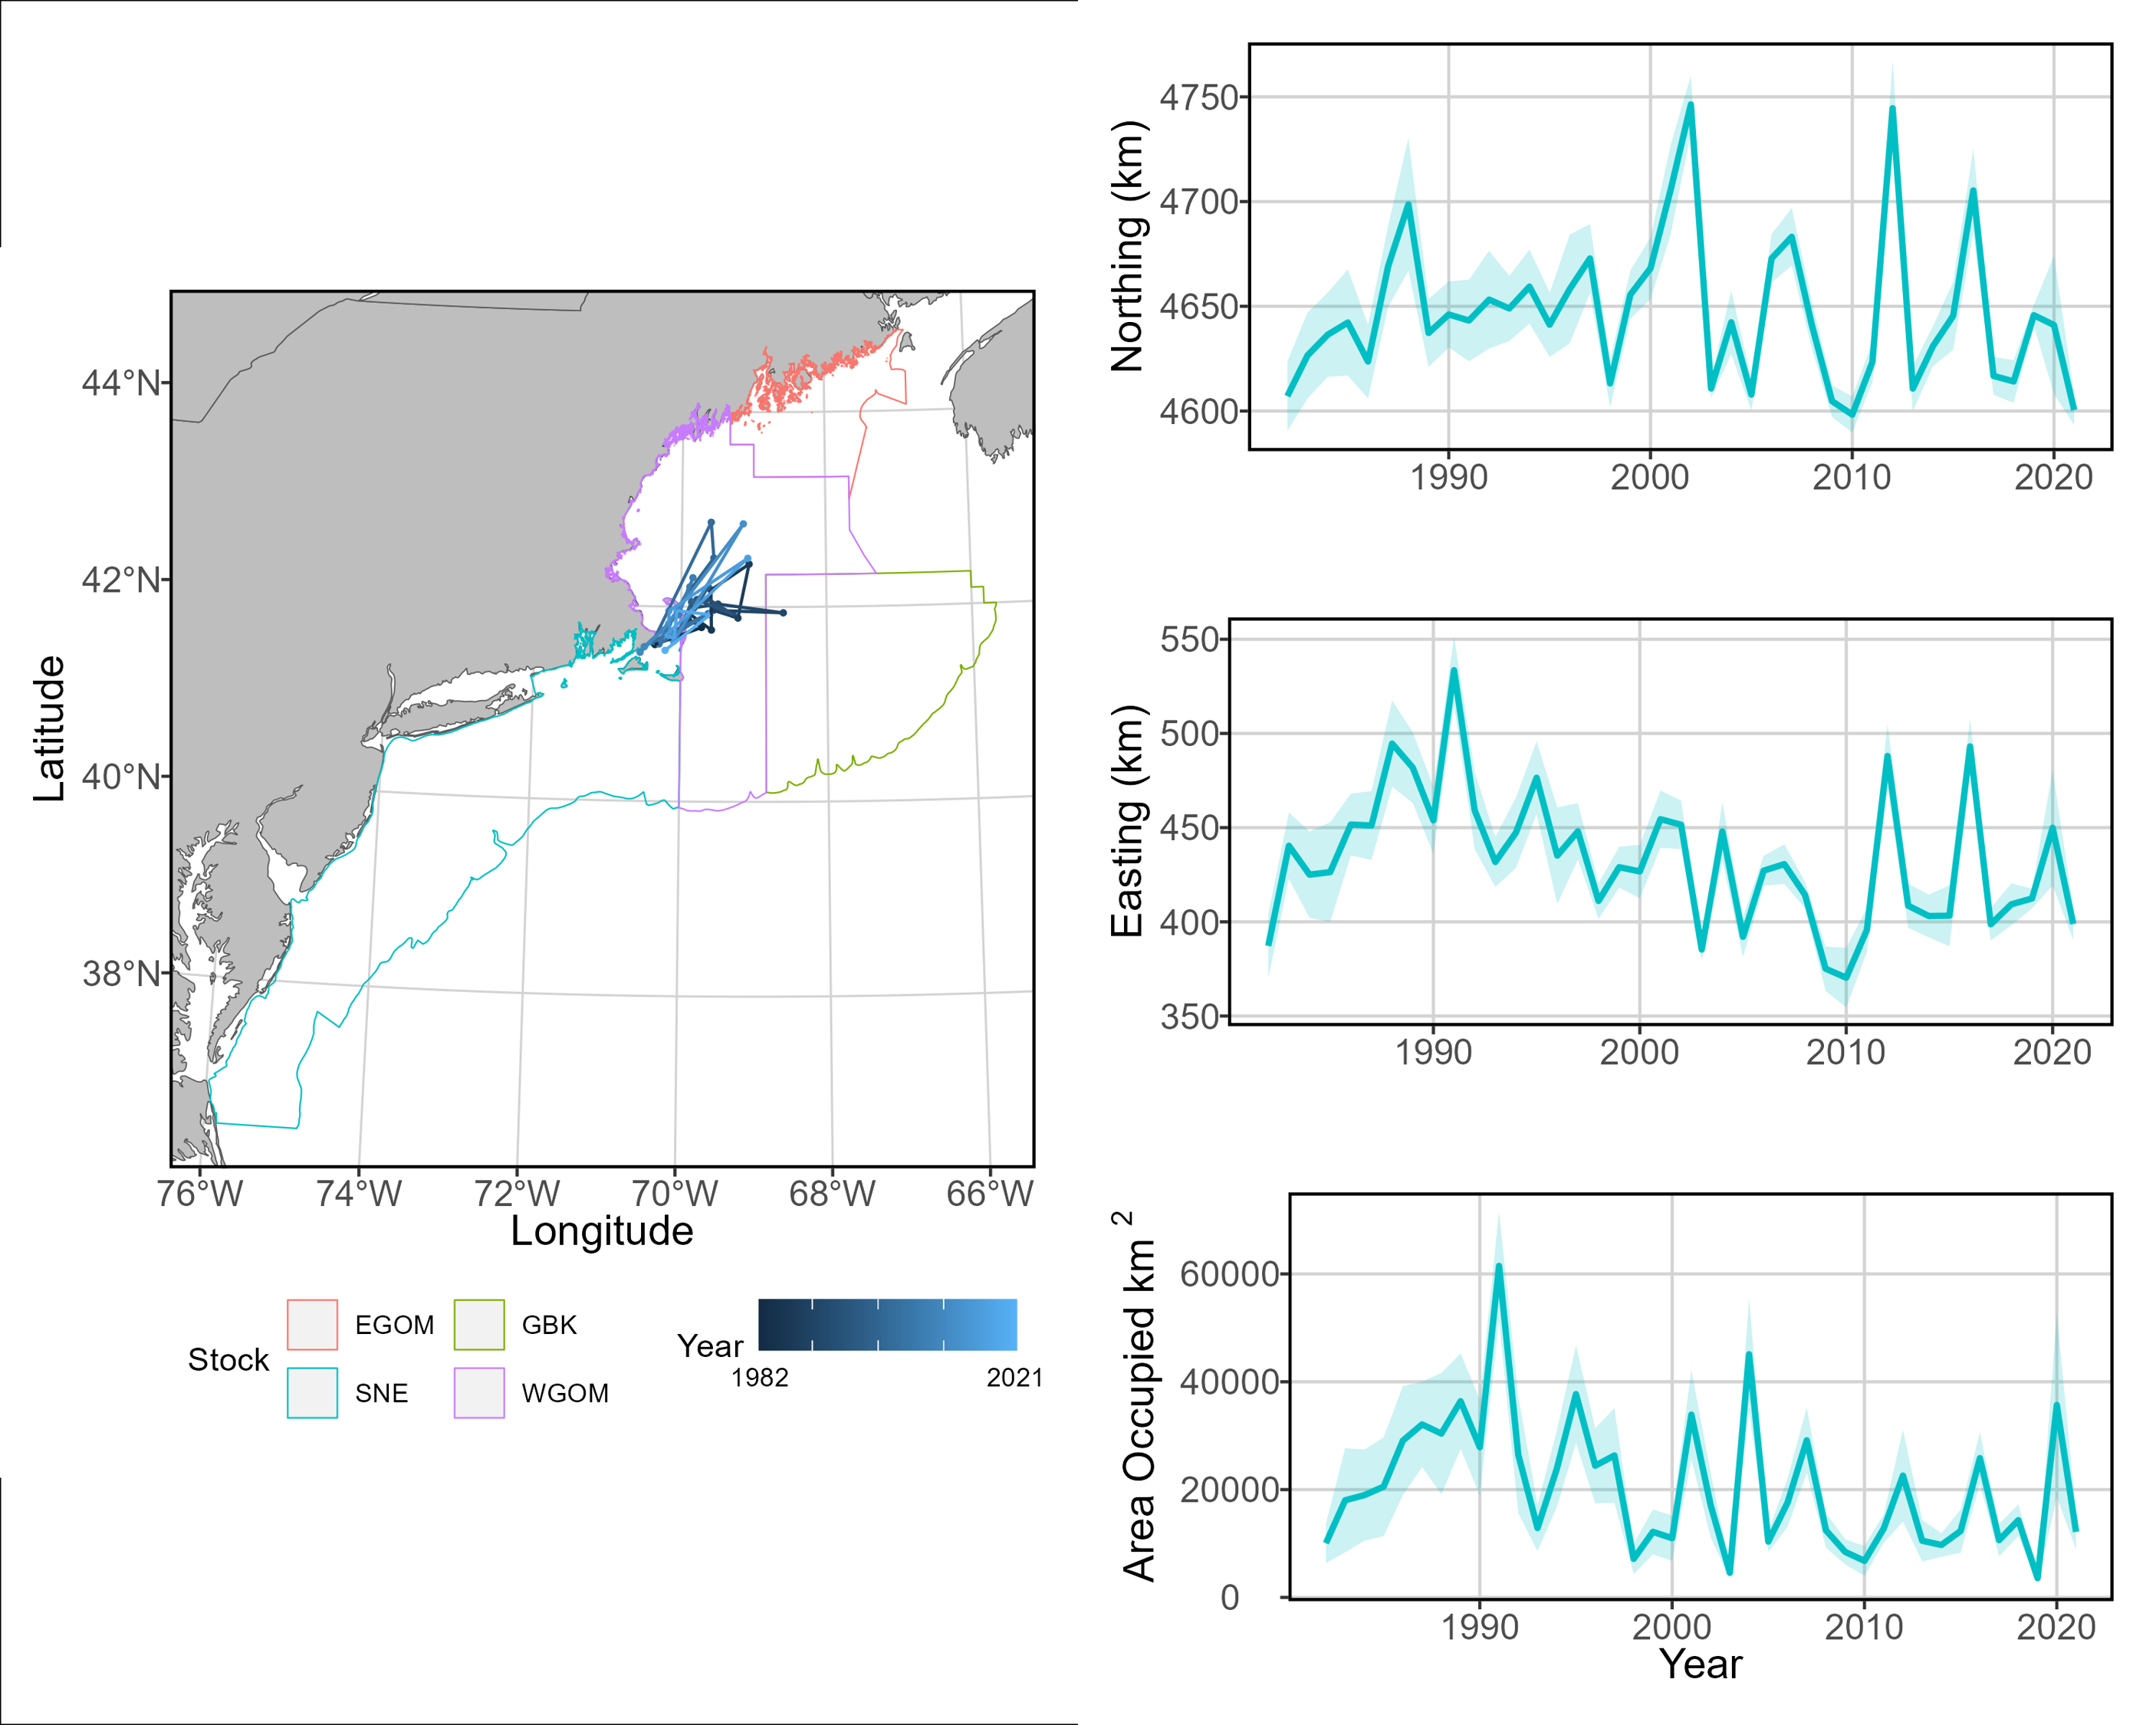
\includegraphics{C:/Users/klankowicz/Documents/GitHub/Atlantic-cod-habitat-VAST/Plot_output_4/small.spring.png}
\caption{Figure 15: Small cod center of gravity and effective area occupied for all stock areas, spring seasons 1982 - 2021.}
\end{figure}

\hypertarget{fall-index}{%
\subsection{Fall Index}\label{fall-index}}

Large cod usually had the lowest abundance within the study area of all three size classes, and abundance for this group decreased over time. This result held for indices calculated within each of the four stock areas as well. Large cod were most abundant in the Georges Bank stock area. The center of gravity for large cod tended to be between the Georges Bank and Western Gulf of Maine stock areas and shifted slightly north over the time series. Effective area occupied decreased dramatically over time.

Medium cod had the highest fall abundance of all size classes, but also had a decreasing abundance trend over time. Similar to large cod, this result held when separating indices of abundance into each of the stock areas. Medium cod were most abundant in the Western Gulf of Maine stock area. The center of gravity for medium cod was typically on the border between the Western Gulf of Maine stock area and the Georges Bank stock area, and moved slightly north over time. Effective area occupied decreased over time.

Unlike the spring indices, small cod did not have high variation in the fall indices. Small cod abundance had a decreasing trend throughout the time but had a rapid fall in abundance in the Southern New England and Western Gulf of Maine stock areas starting around 2010. The center of gravity for small cod was in the Western Gulf of Maine stock area, and there is no clear trend in movement over time. There is also no clear trend for changes in effective area occupied over time.

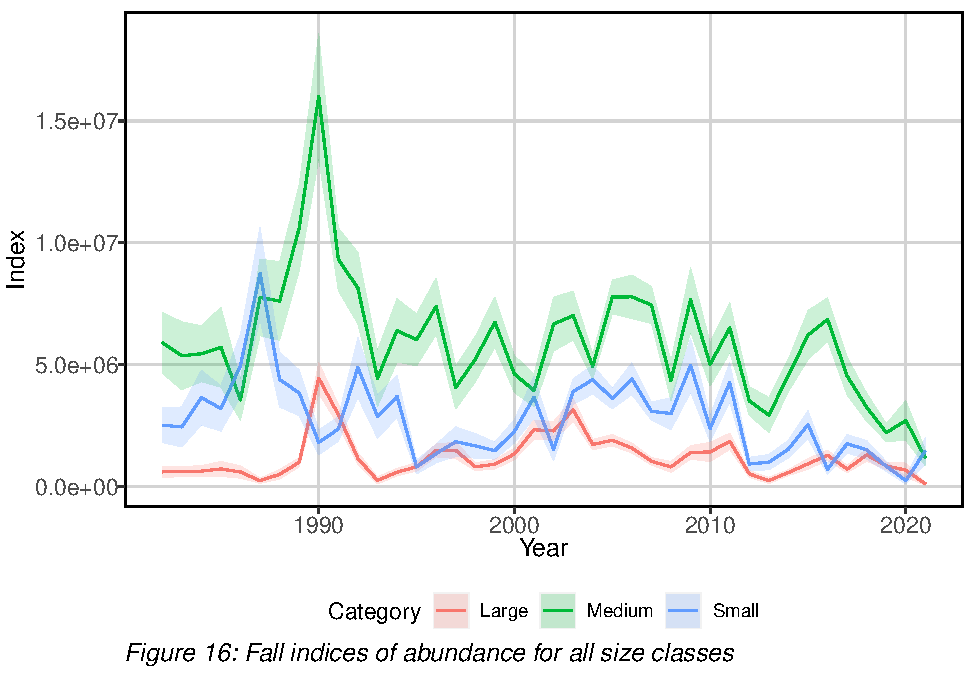
\includegraphics{ToR1_TechPaper_files/figure-latex/fall index-1.pdf} 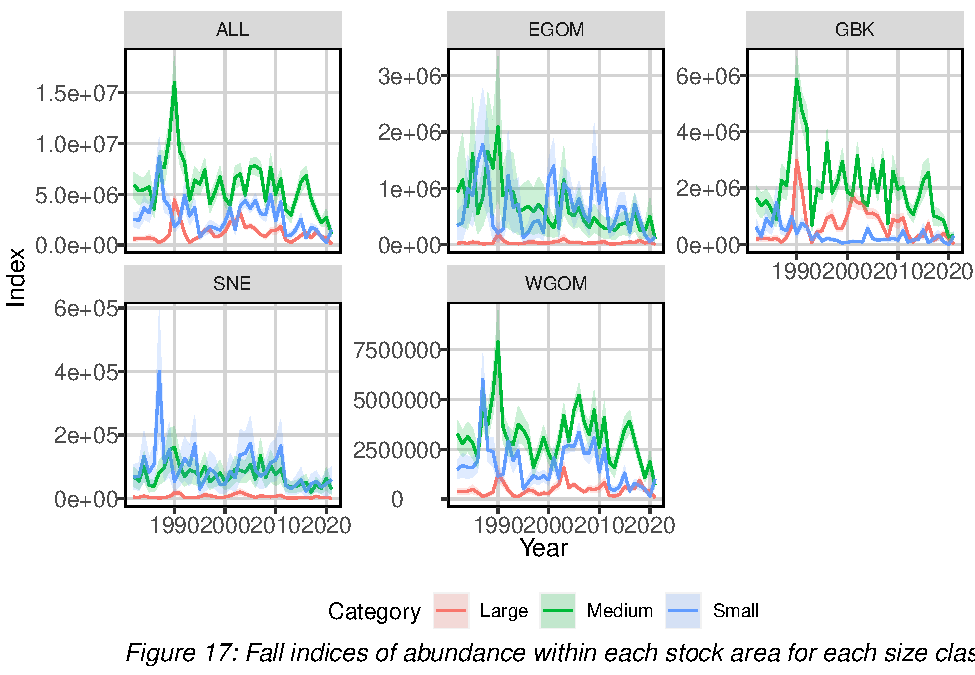
\includegraphics{ToR1_TechPaper_files/figure-latex/fall index-2.pdf}

\begin{figure}
\centering
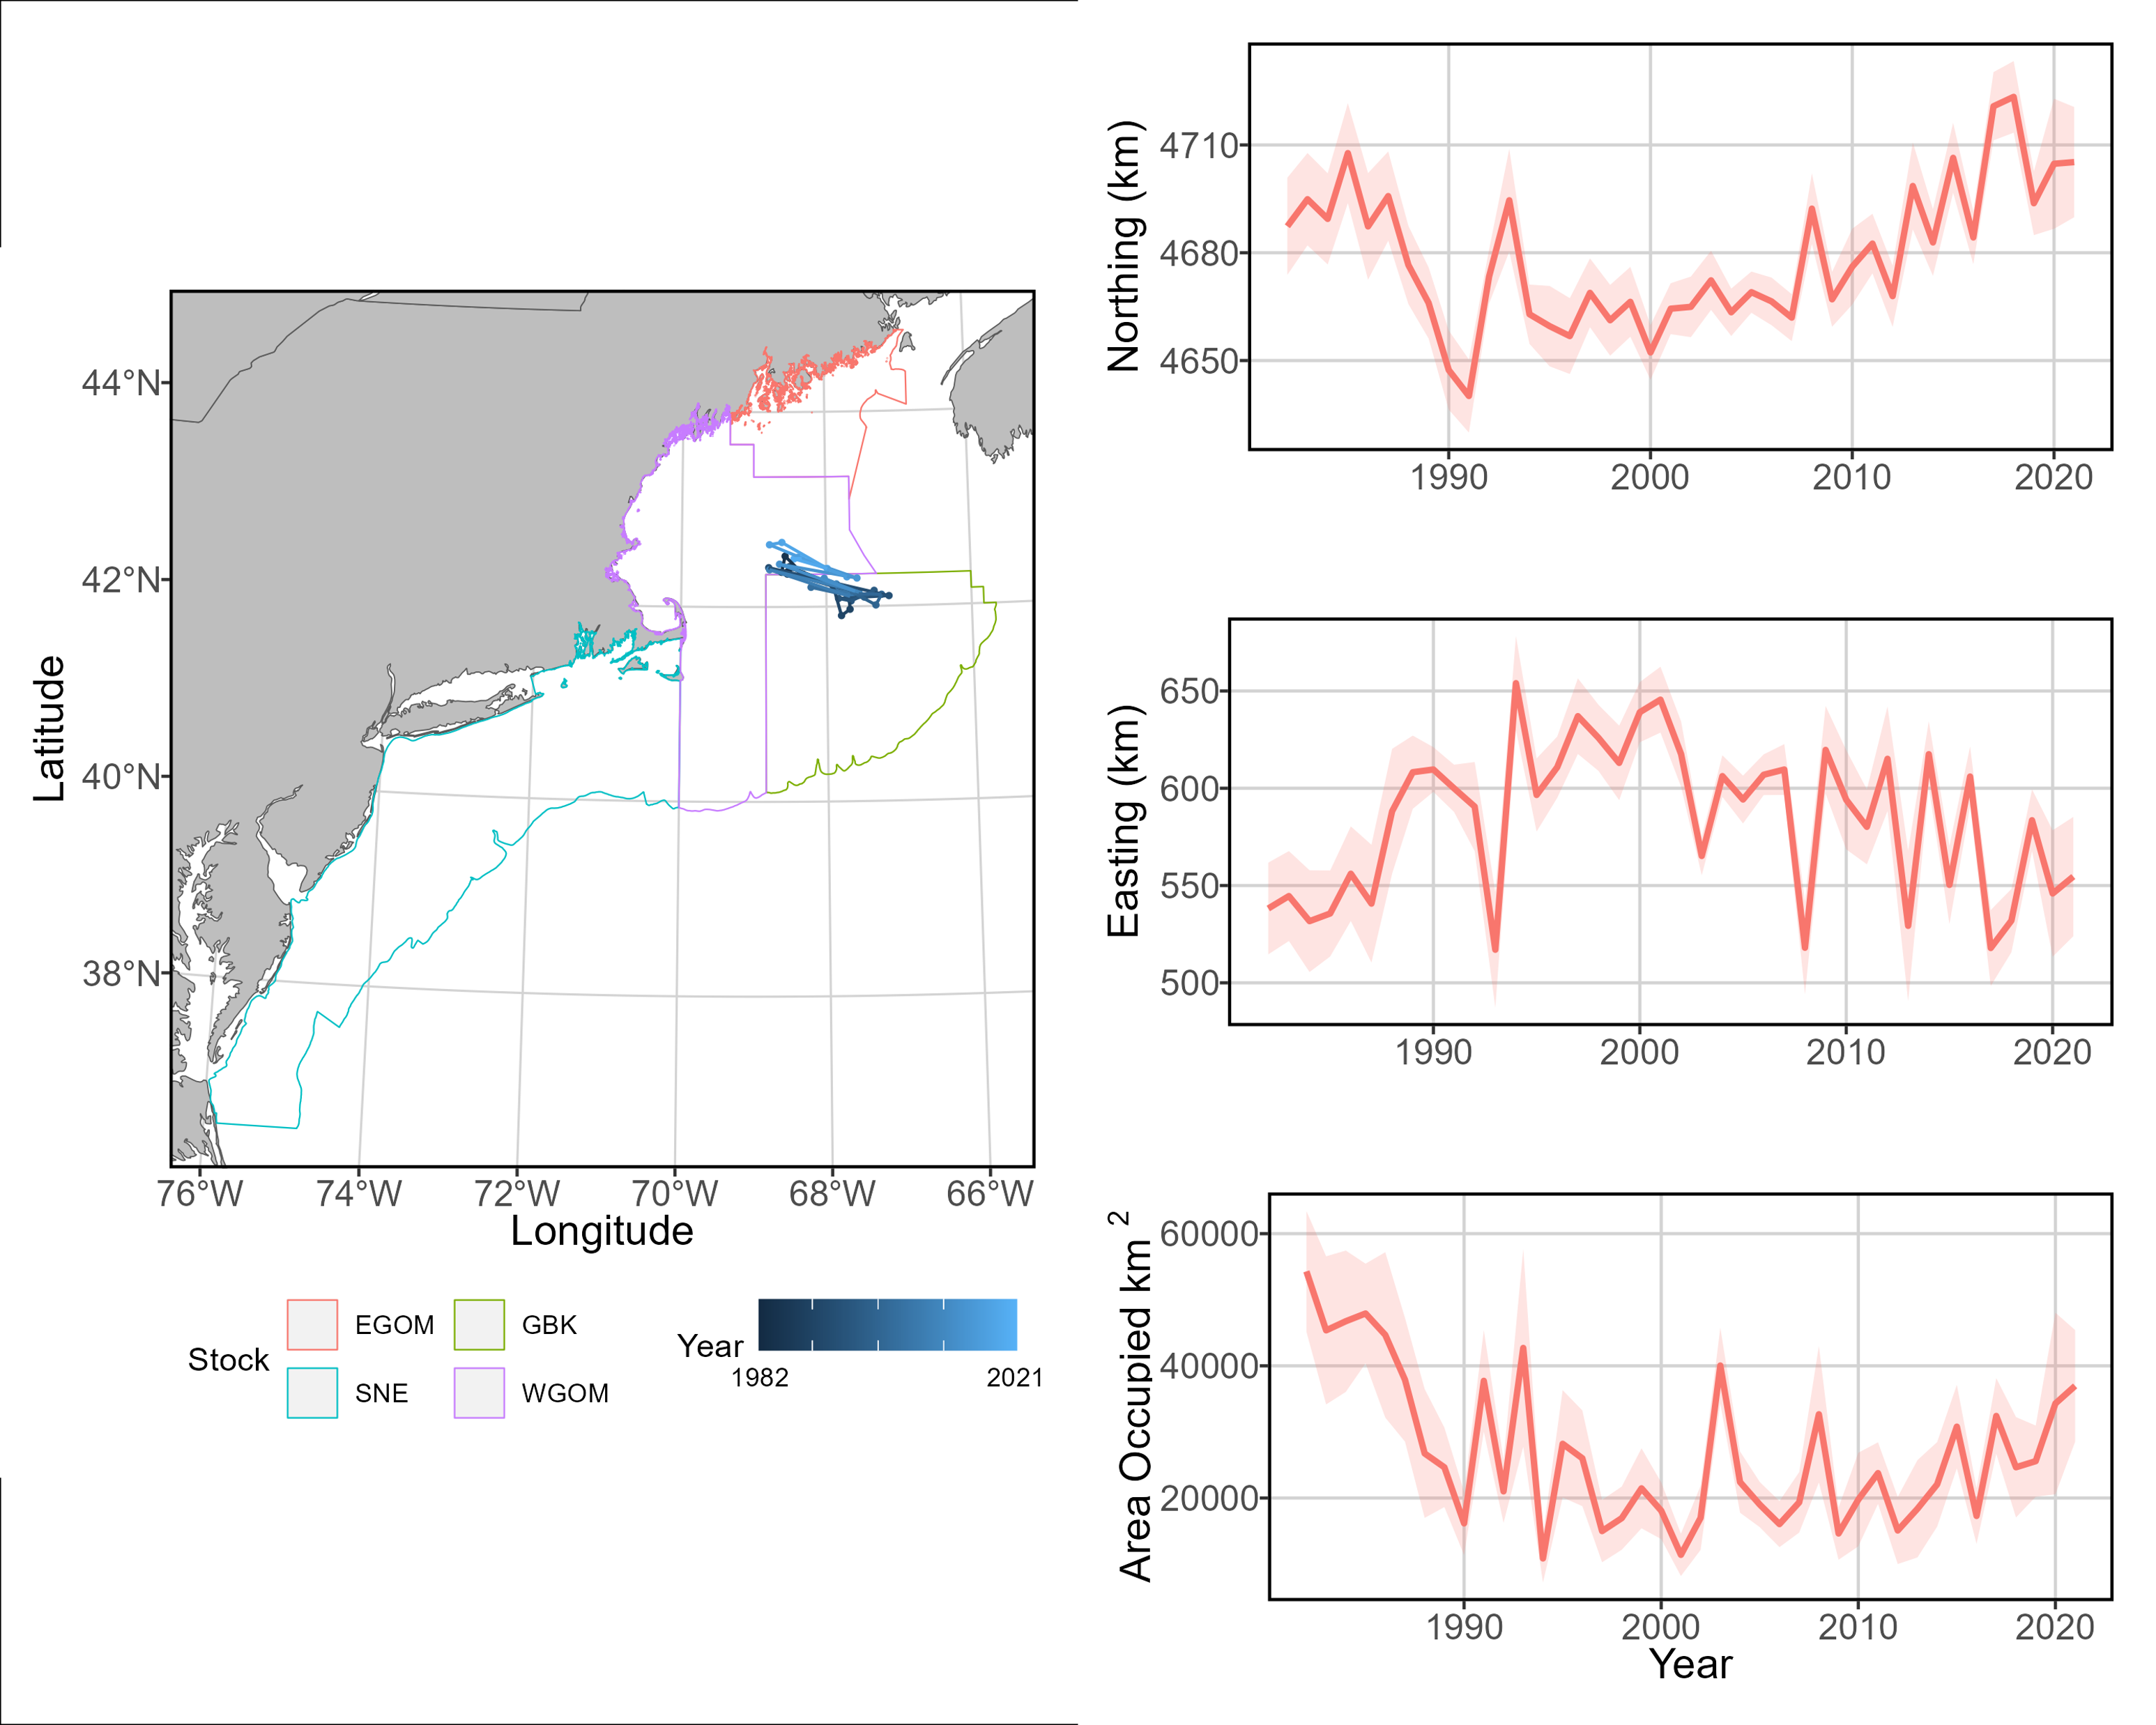
\includegraphics{C:/Users/klankowicz/Documents/GitHub/Atlantic-cod-habitat-VAST/Plot_output_4/large.fall.png}
\caption{Figure 18: Large cod center of gravity and effective area occupied for all stock areas, fall seasons 1982 - 2021.}
\end{figure}

\begin{figure}
\centering
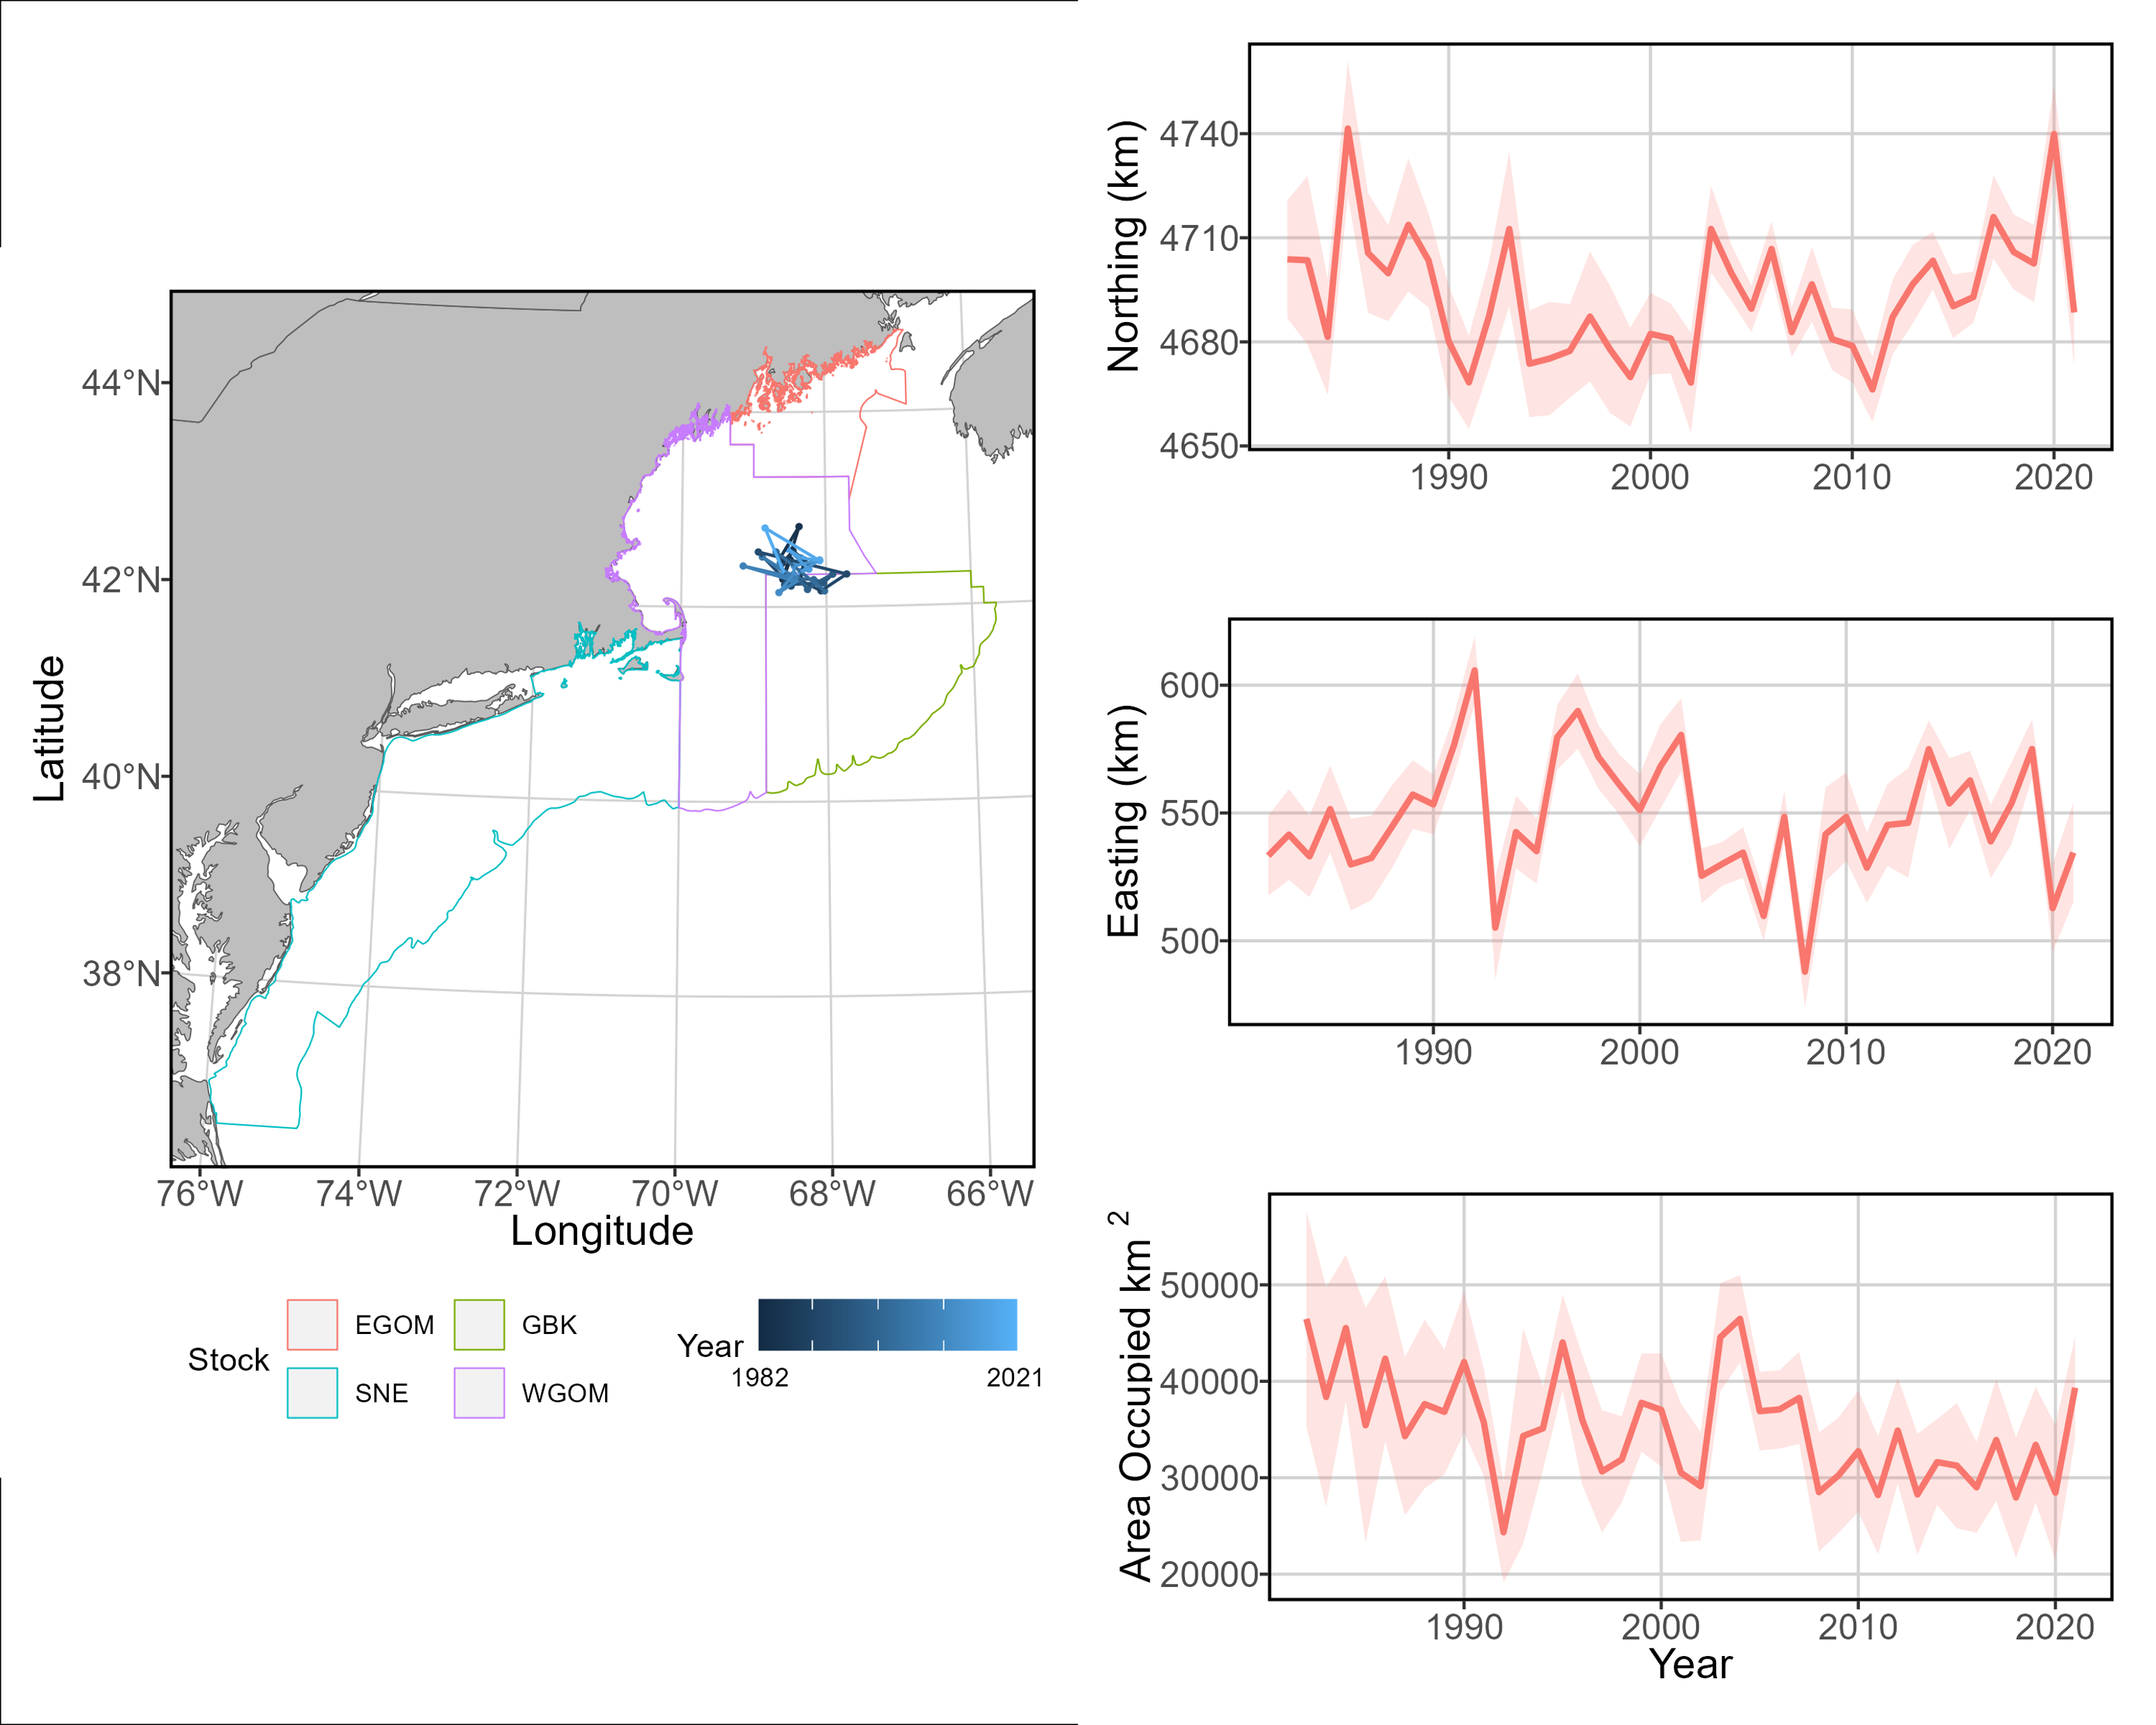
\includegraphics{C:/Users/klankowicz/Documents/GitHub/Atlantic-cod-habitat-VAST/Plot_output_4/medium.fall.png}
\caption{Figure 19: Medium cod center of gravity and effective area occupied for all stock areas, fall seasons 1982 - 2021.}
\end{figure}

\begin{figure}
\centering
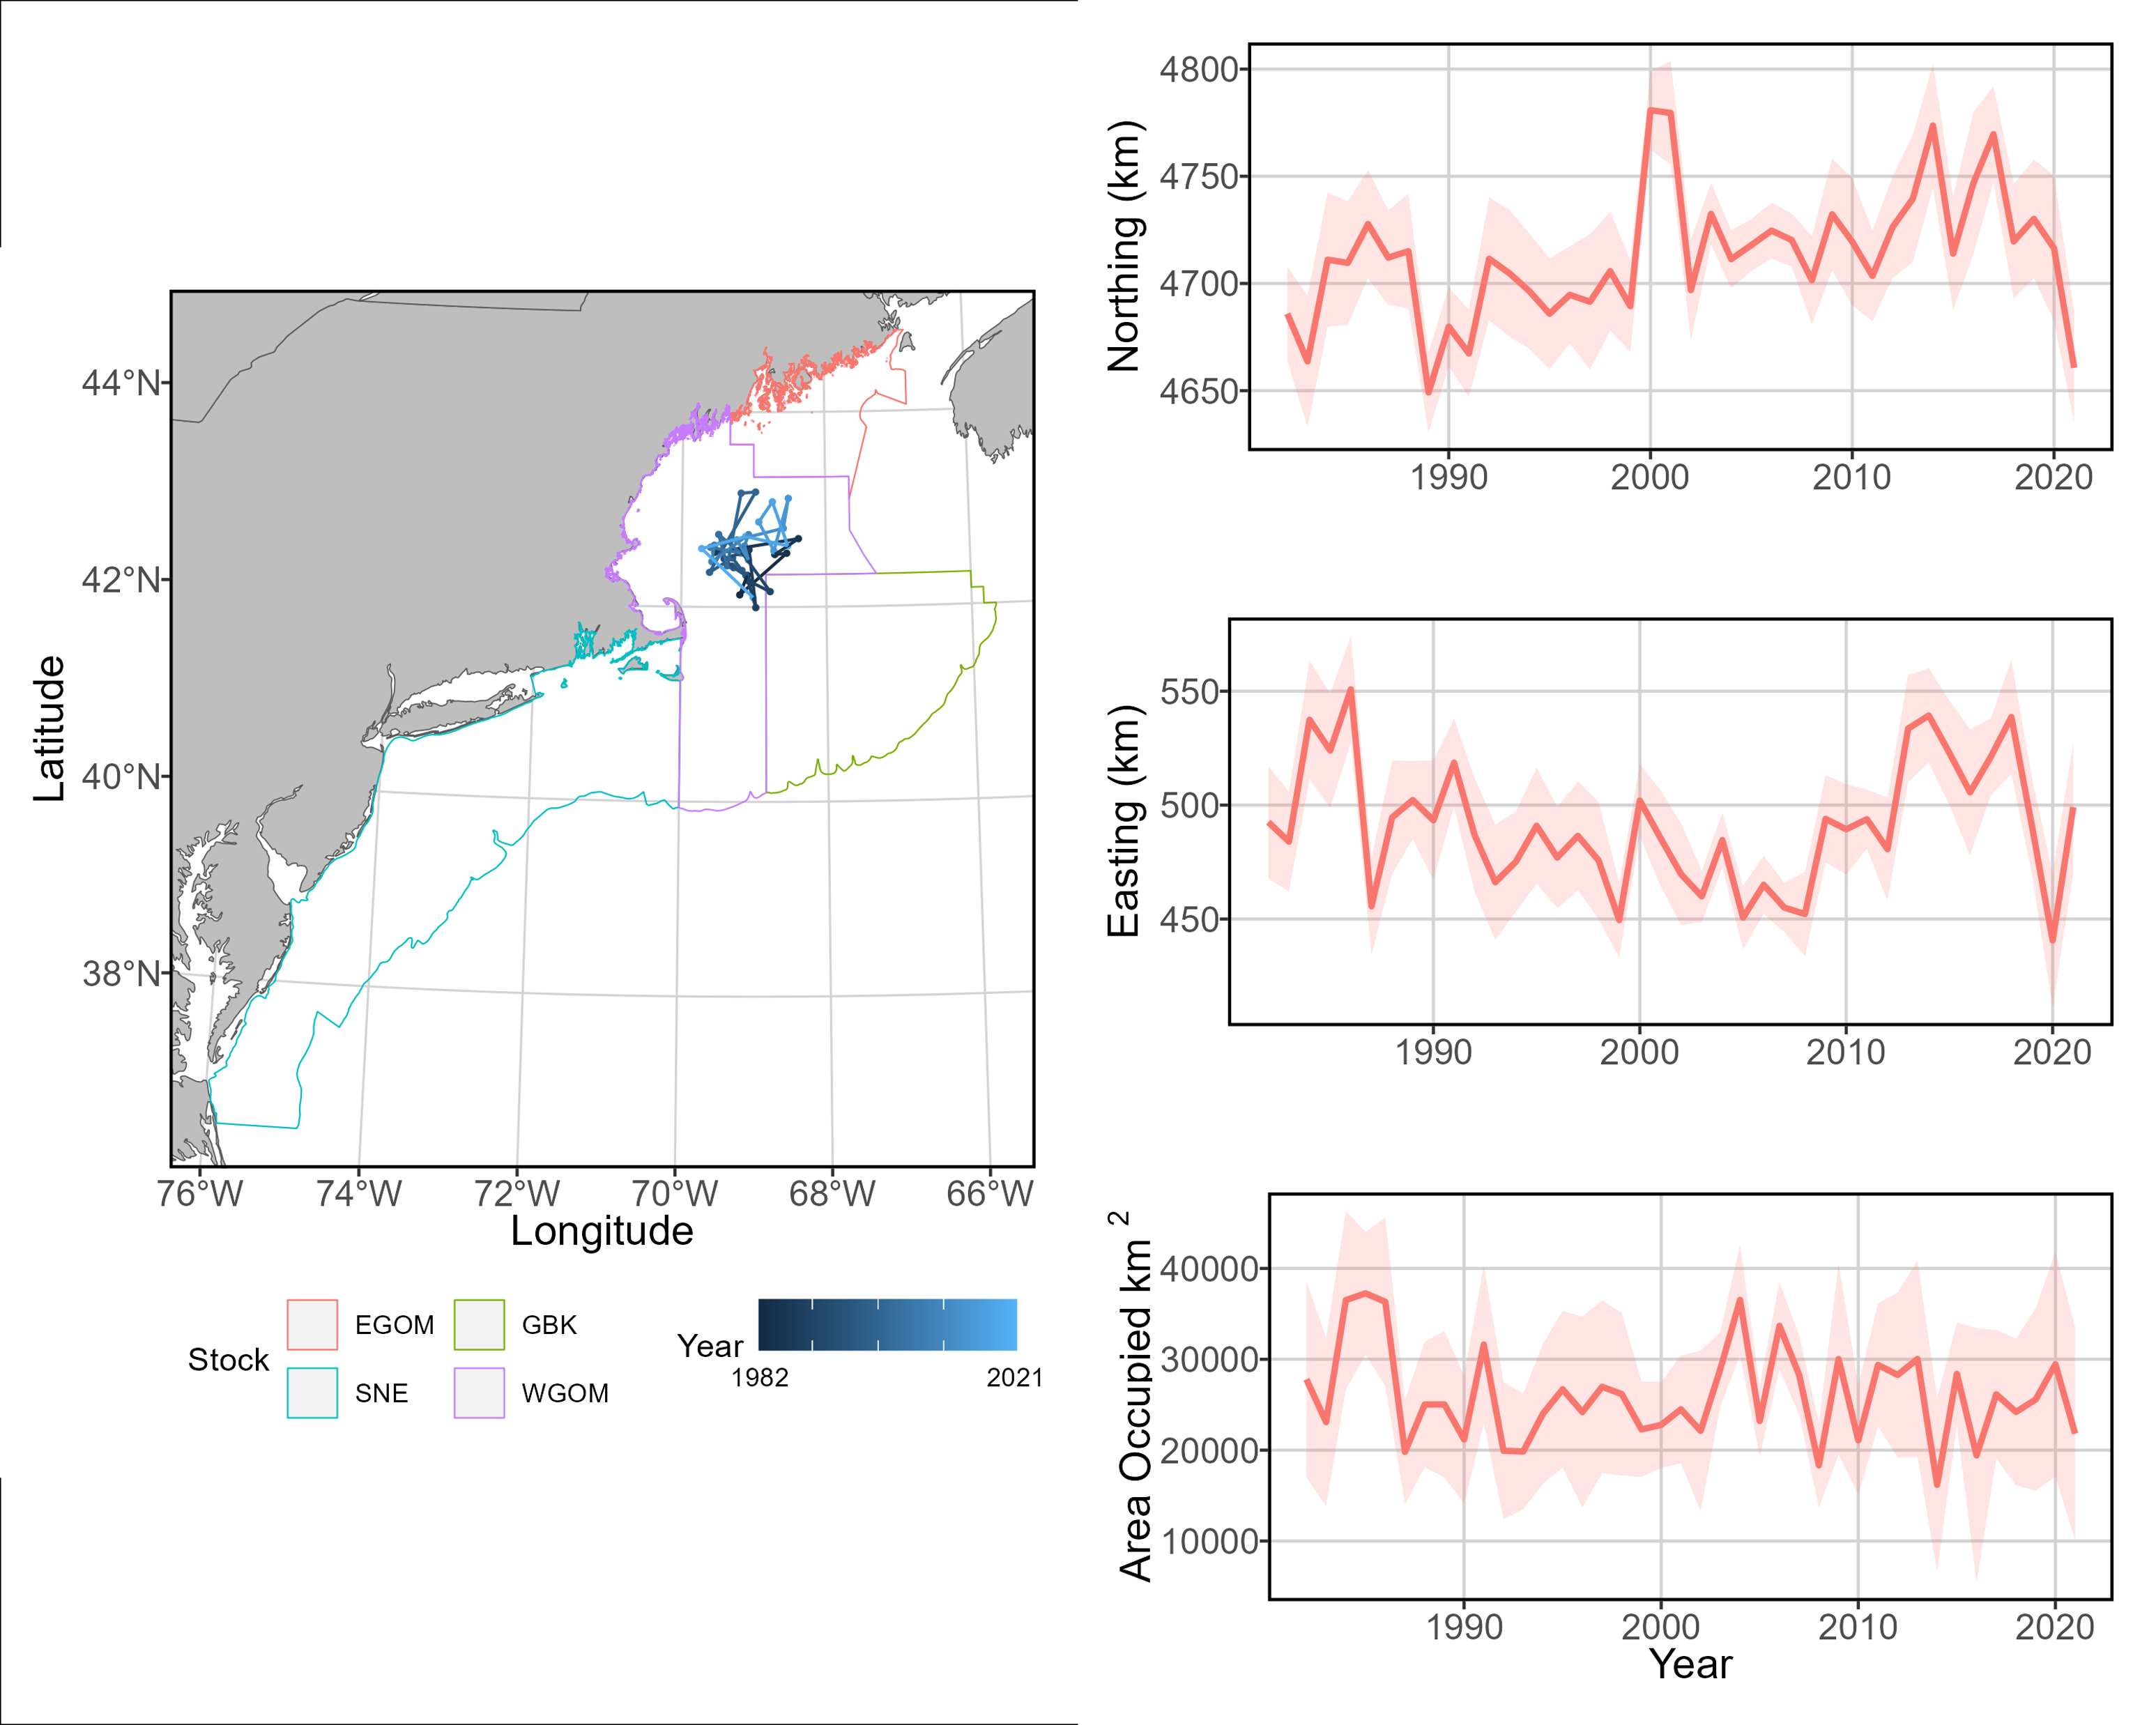
\includegraphics{C:/Users/klankowicz/Documents/GitHub/Atlantic-cod-habitat-VAST/Plot_output_4/small.fall.png}
\caption{Figure 20: Small cod center of gravity and effective area occupied for all stock areas, fall seasons 1982 - 2021.}
\end{figure}

\hypertarget{habitat-associations}{%
\subsection{Habitat associations}\label{habitat-associations}}

After modeling, VAST extrapolation grid cells were stratified into hard, mixed, and soft bottom types using k-means clustering. Soft-bottom grid cells most likely contained only mud or sand, mixed-bottom cells contained similar likelihoods of mud, sand, and gravel, and hard-bottom grid cells likely contained cobble. The resulting map of sediment ``hardness'' was plotted with the aggregate spatial density of each cod size class for the spring and fall time series.

Small cod were highly concentrated in nearshore waters around Martha's Vineyard and Narragansett Bay during the spring season, and more concentrated in nearshore waters around Boston Harbor in the fall. They were not strongly associated with any sediment type, though areas of high abundance in the fall were typically in areas of mixed sediment. Medium cod were more generally spread throughout the Gulf of Maine, and were typically found in highest density in areas of mixed sediment type. Large cod were highly dense in much smaller spatial areas. In the spring, this density was concentrated at the eastern end of Georges Bank and within areas of mixed sediment type. In the fall, large cod density was highest in the waters around the Westen Gulf of Maine closed area and within habitats of either mixed or hard sediment type.

\begin{figure}
\centering
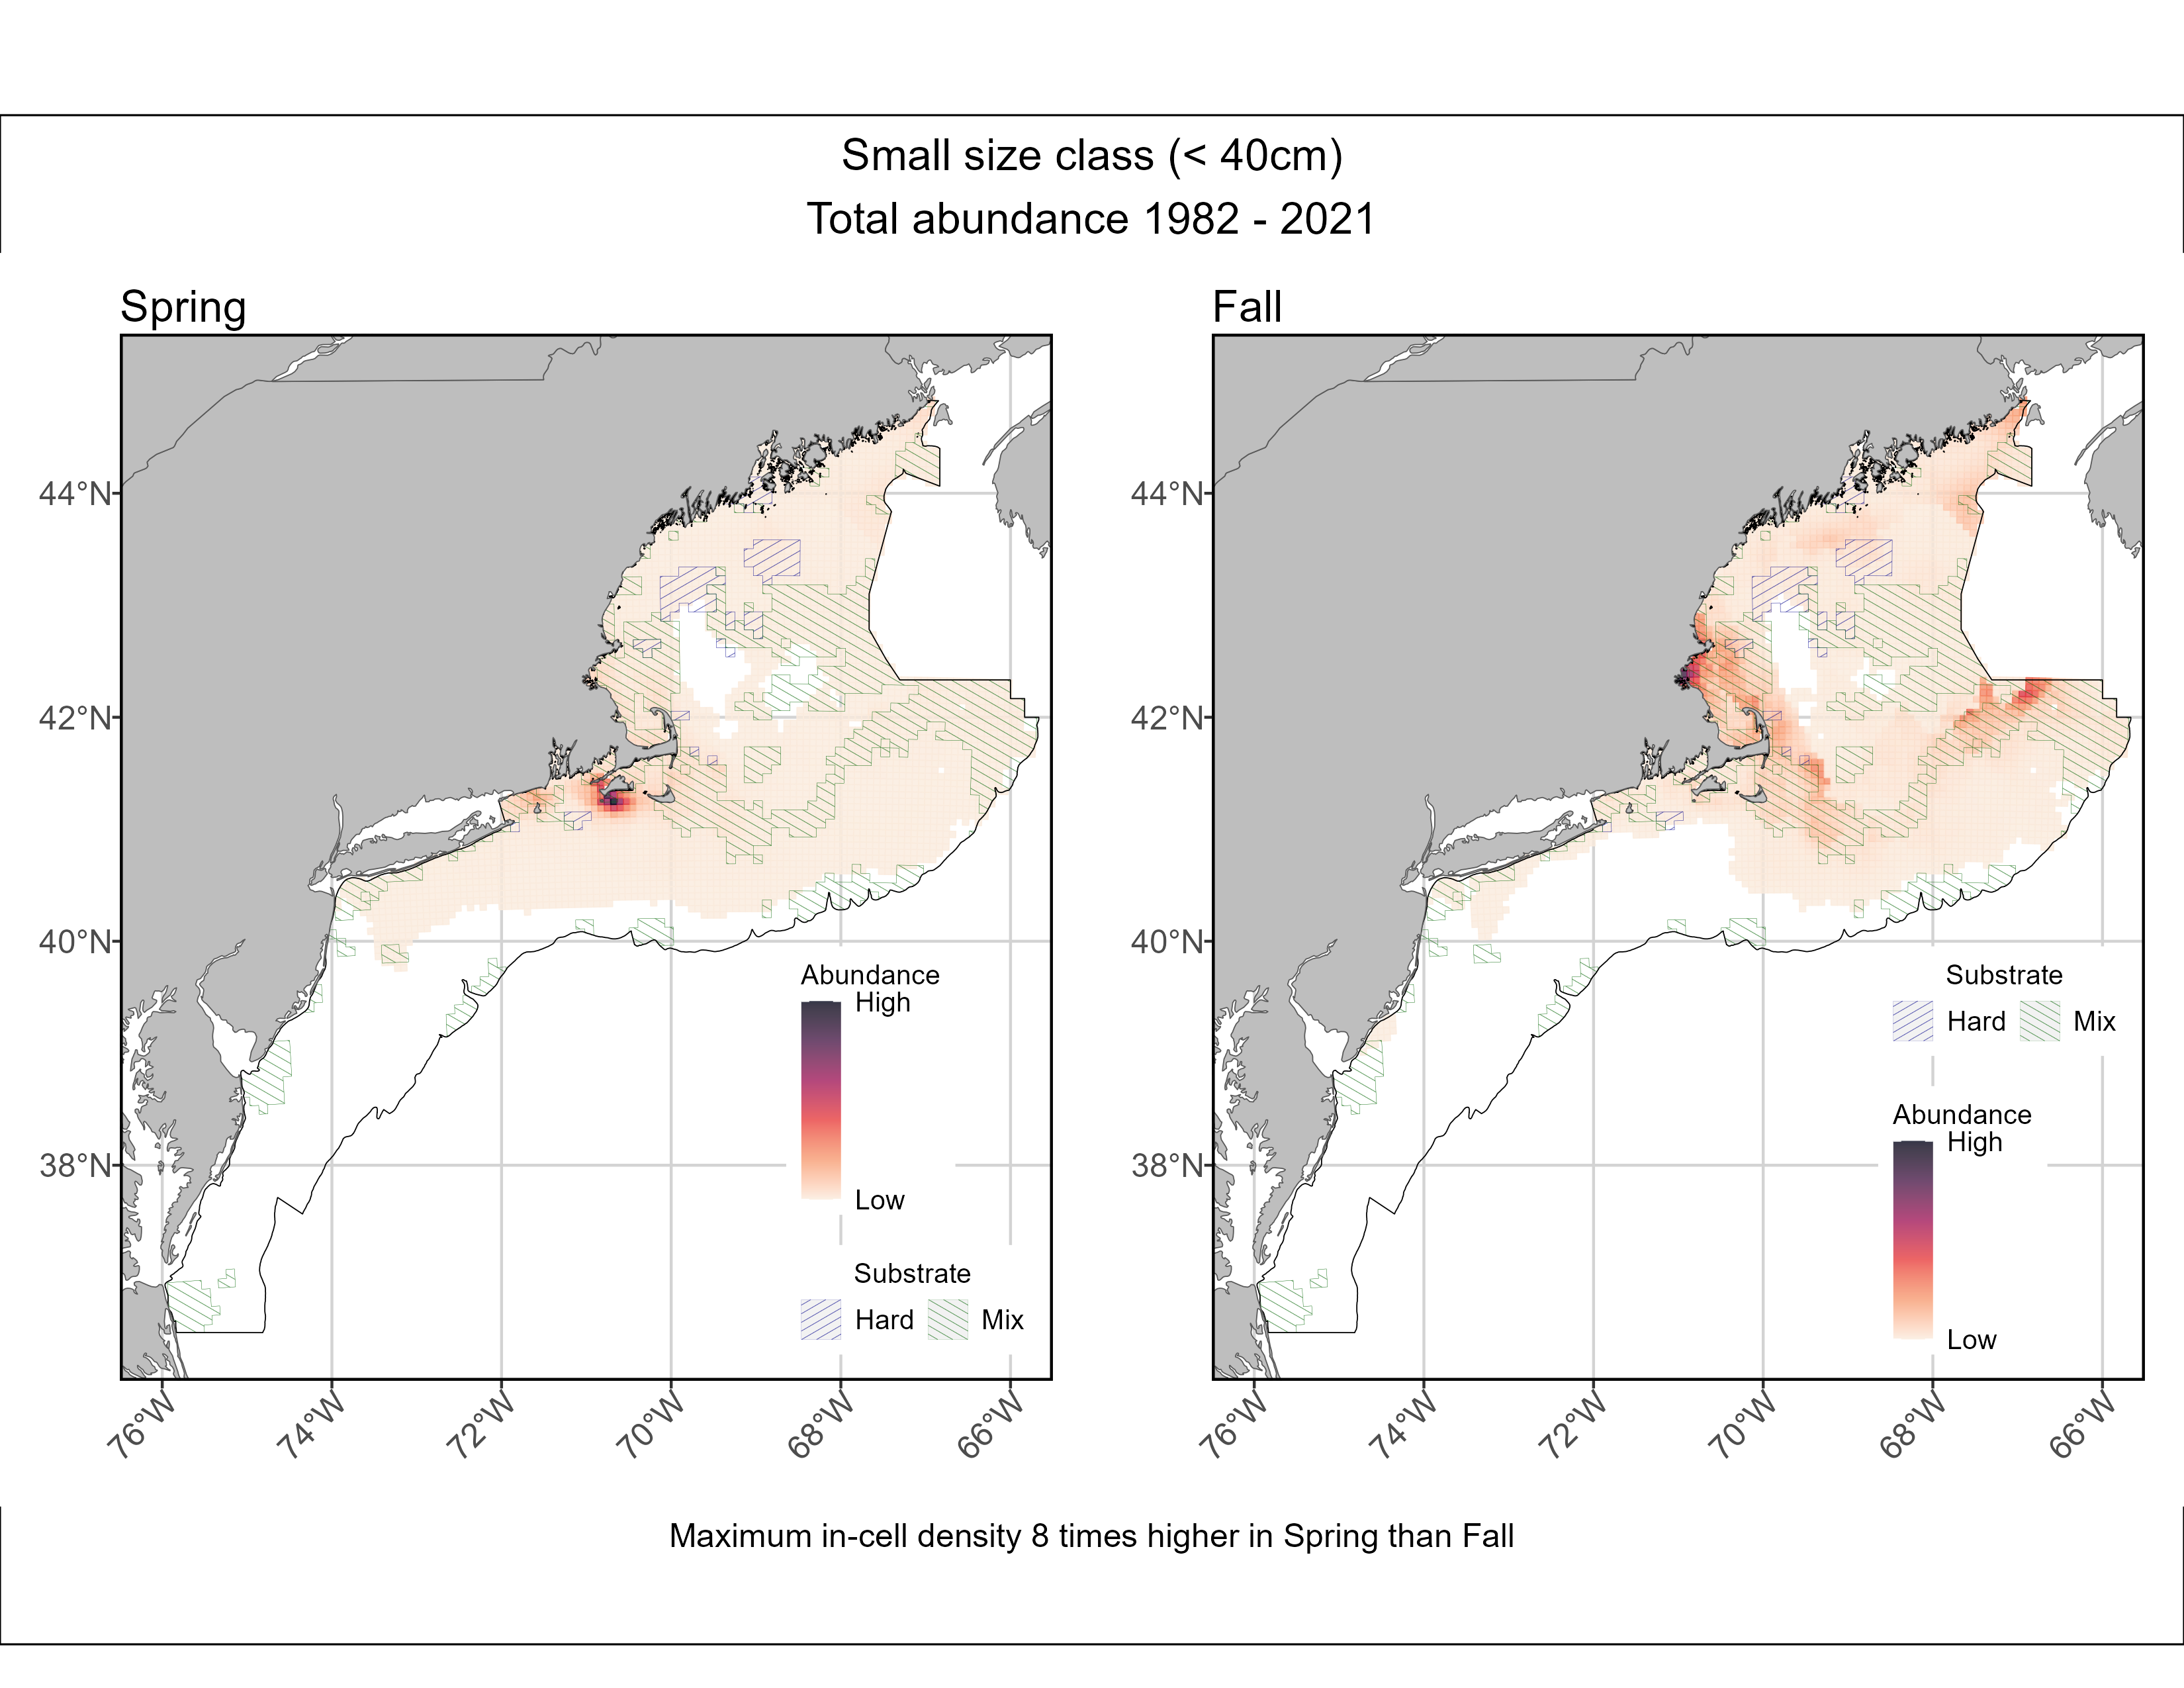
\includegraphics{C:/Users/klankowicz/Documents/GitHub/Atlantic-cod-habitat-VAST/Plot_output/total_spatialdensity_small.png}
\caption{Figure 21: Small cod aggregate spatial density split by season, 1982 - 2021.}
\end{figure}

\begin{figure}
\centering
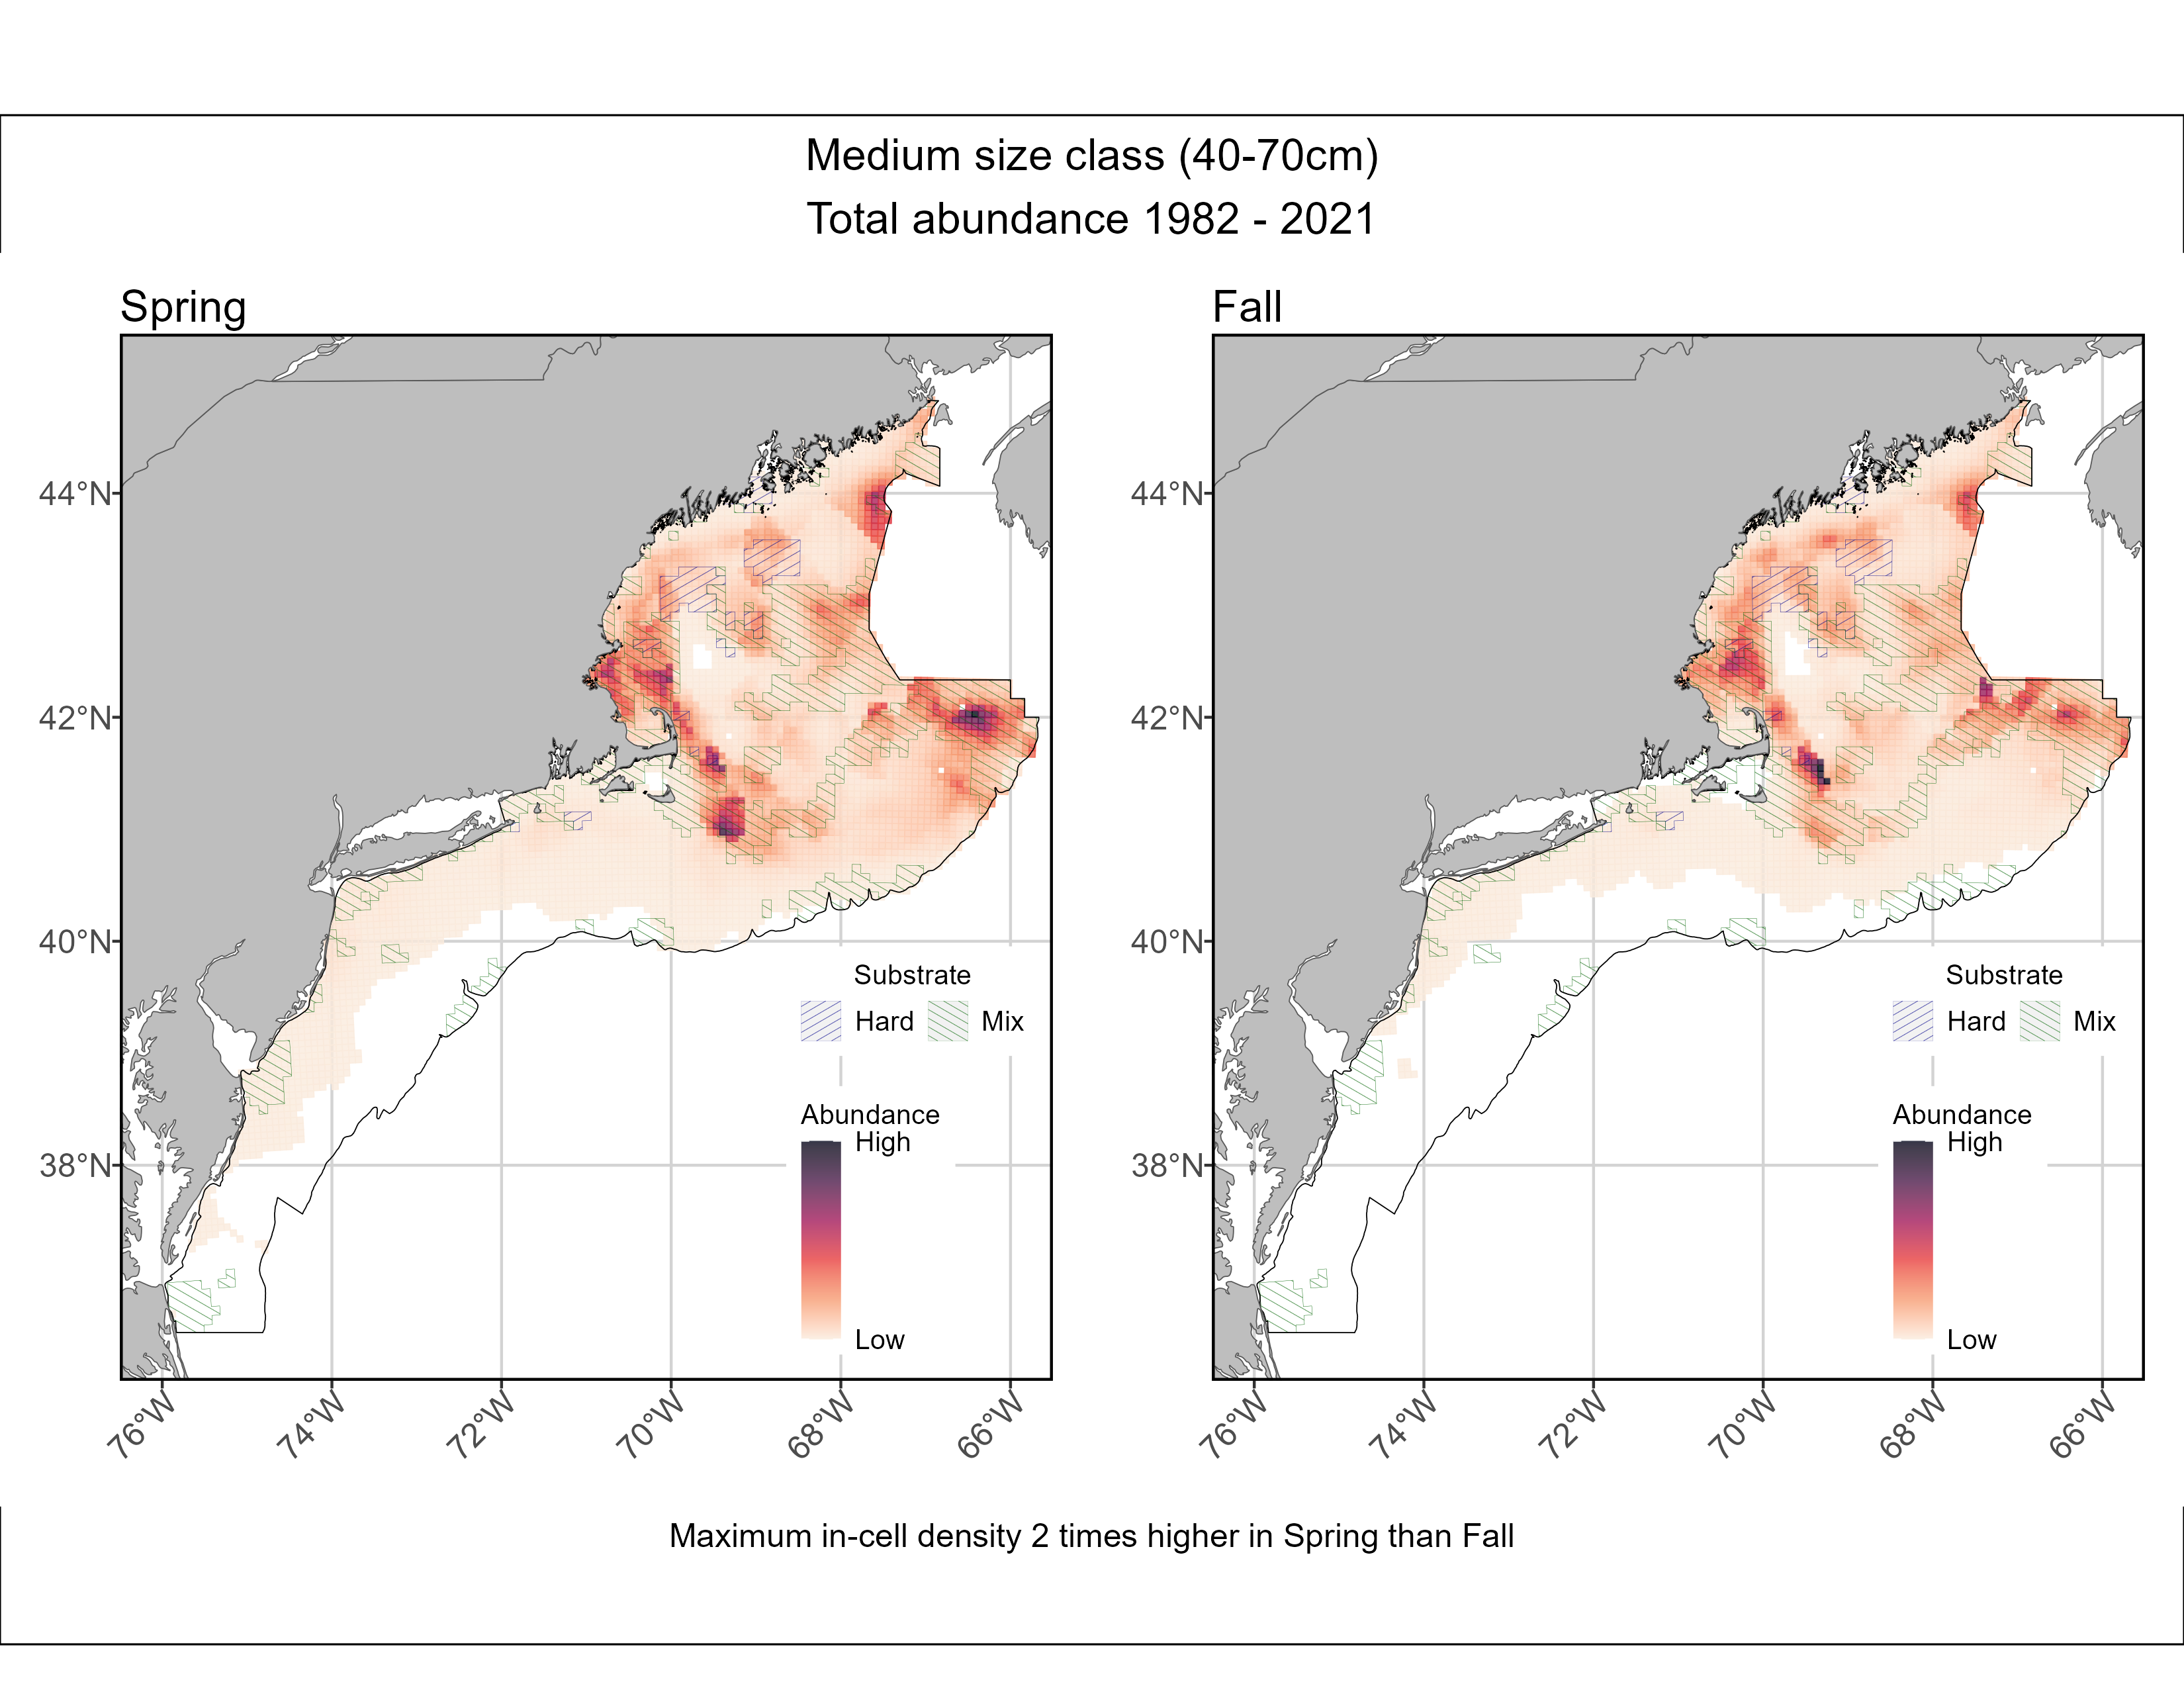
\includegraphics{C:/Users/klankowicz/Documents/GitHub/Atlantic-cod-habitat-VAST/Plot_output/total_spatialdensity_medium.png}
\caption{Figure 22: Medium cod aggregate spatial density split by season, 1982 - 2021.}
\end{figure}

\begin{figure}
\centering
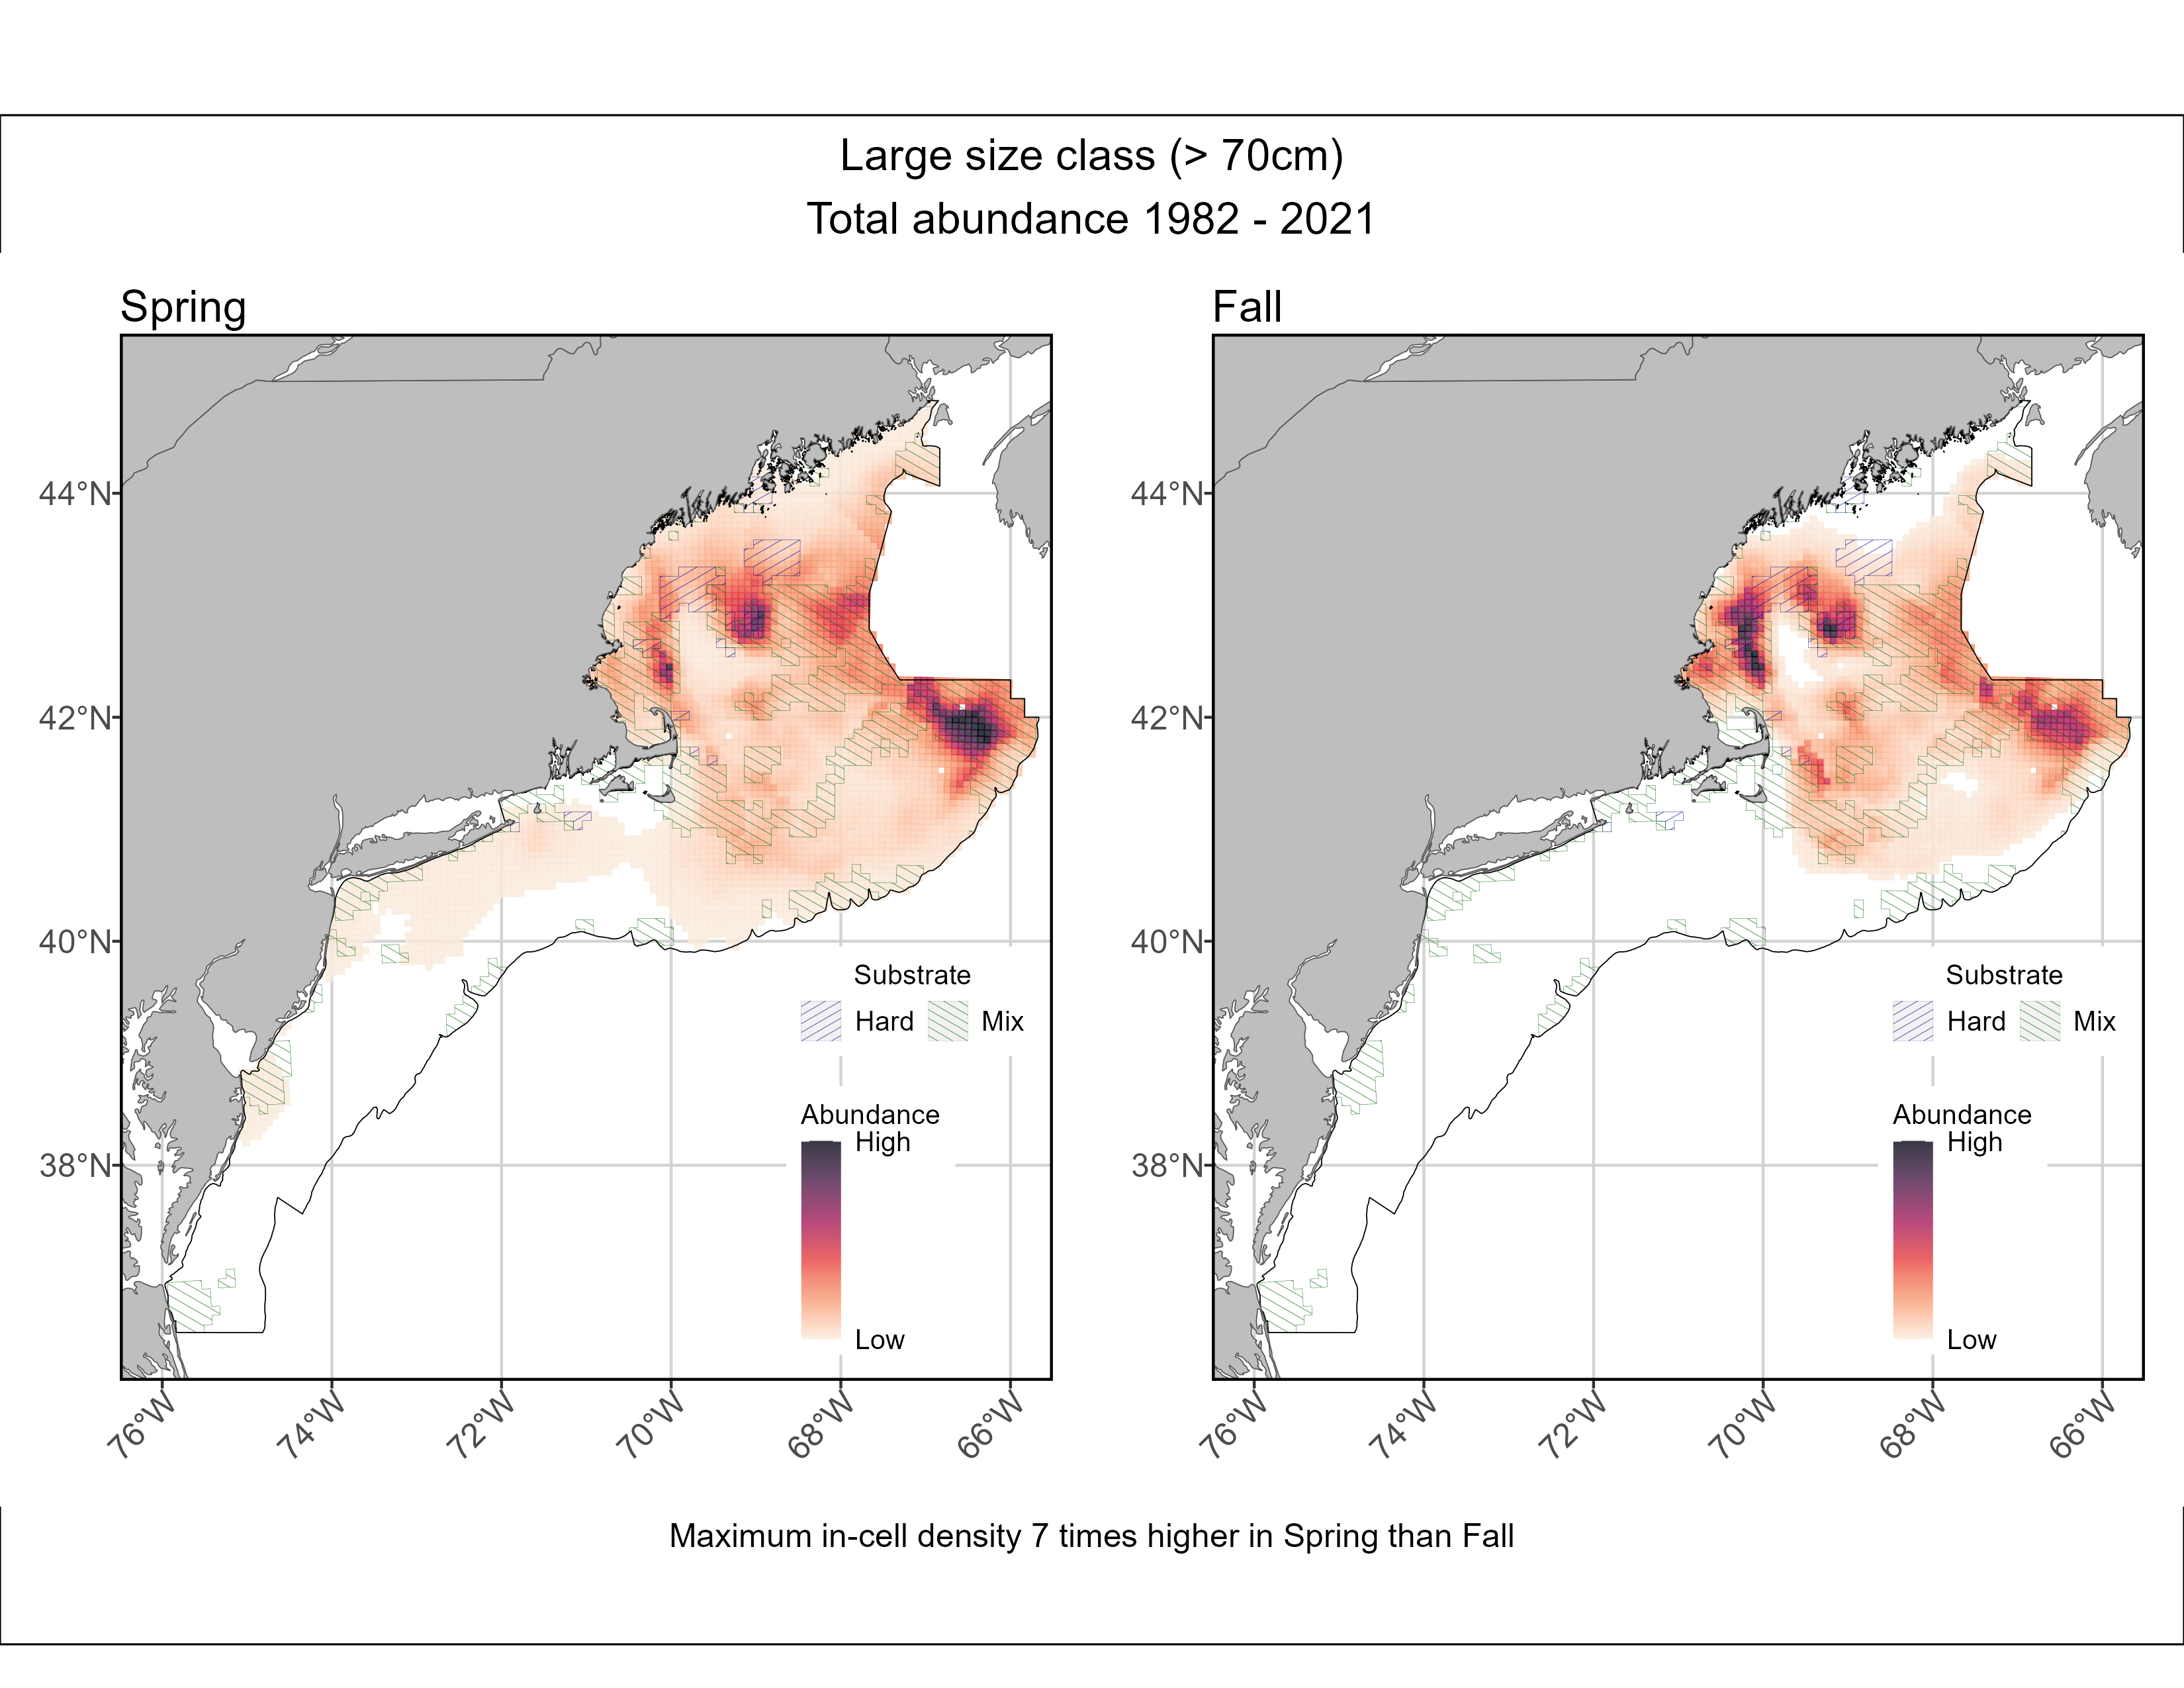
\includegraphics{C:/Users/klankowicz/Documents/GitHub/Atlantic-cod-habitat-VAST/Plot_output/total_spatialdensity_large.png}
\caption{Figure 23: Large cod aggregate spatial density split by season, 1982 - 2021.}
\end{figure}

\hypertarget{model-diagnostics}{%
\subsection{Model diagnostics}\label{model-diagnostics}}

The effect of anisotropy was stronger in the first linear predictor than the second, meaning that probability of encountering cod was similar for longer distances along a northeast-to-southwest axis than the abundance of cod along the same axis.

\begin{figure}
\centering
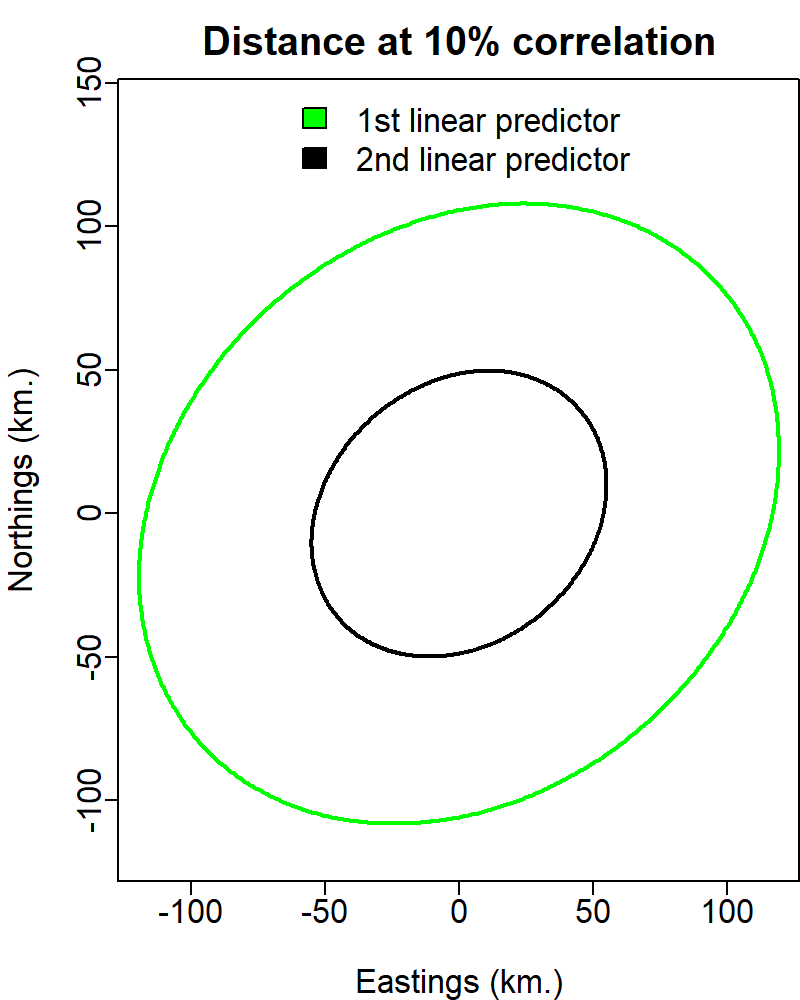
\includegraphics{C:/Users/klankowicz/Documents/GitHub/Atlantic-cod-habitat-VAST/VAST_runs/add_climate_aja4/GBK/Aniso.png}
\caption{Figure 24: Anisotropic effect in the first and second linear predictors}
\end{figure}

Residual plots did not indicate any violation of assumptions in the construction or implementation of the model. Mapping residuals within the model spatial domain did not highlight any spatial area as having a consistently poor fit.

\begin{figure}
\centering
\includegraphics{C:/Users/klankowicz/Documents/GitHub/Atlantic-cod-habitat-VAST/VAST_runs/add_climate_aja4/GBK/Quantile_residuals.png}
\caption{Figure 25: Quantile residuals of model run}
\end{figure}

\begin{figure}
\centering
\includegraphics{C:/Users/klankowicz/Documents/GitHub/Atlantic-cod-habitat-VAST/VAST_runs/add_climate_aja4/GBK/Quantile_residuals_on_map.png}
\caption{Figure 26: Quantile residuals of model run in spatial domain for every time step}
\end{figure}

\hypertarget{discussion}{%
\section{Discussion}\label{discussion}}

Currently, groundfish population assessments rely heavily on data gathered with bottom trawl surveys. Despite evidence of increased cod abundance in areas with complex bottom habitats, locations with large-grain sediments or high rugosity are avoided or sampled at low frequency with bottom trawls due to the risks of damaging equipment. This is a major point of contention for fishing industry members, who believe that limiting information from complex habitats will not accurately reflect cod spatial distribution or abundance (\protect\hyperlink{ref-grabowski_2020}{Grabowski et al. 2020}). Industry members instead support sampling across all habitat types and utilizing dynamic stratification, in which areas of similar habitat characteristics and likelihood of encountering cod are grouped into strata for sampling and later inclusion in assessment efforts. These strata cannot be built without accurate information on cod spatial density for all habitats within their spatial range.

VAST models can provide a flexible but robust framework to better assess groundfish populations across all habitat types within their spatial ranges. This is, of course, reliant on the collection of survey data in areas typically not well sampled by bottom trawls and by high-quality environmental and habitat data as density covariates.The model of cod spatial density created in this project utilized observation data from a suite of gear types and survey platforms, which bridged some of the data gaps inherent to models built with only bottom trawl survey data. The VAST modeling framework allowed for the use of density covariates to interpolate cod spatial density in non-sampled areas with known habitat and environmental characteristics. Further, VAST allowed for the estimation of spatial, temporal, and spatiotemporal correlation of cod abundance, as well as the inclusion of vessel effects, to facilitate the combination of observation data from multiple sources with varied protocols. This modeling process may be more favorable to industry stakeholders than models built with only bottom trawl observation data.

VAST models highlighted the variable spatial density of cod size classes across the four stock areas within the model spatial domain. There was a clear north-south directional gradient of abundance linked to size, where small cod were most abundant furthest south among the size classes and large cod were most abundant furthest north among the size classes. Further, VAST results highlighted the importance of relatively small areas within the stock areas to the size classes of cod. For example, the importance of Georges Bank to the large size class was highlighted; in the spring season, large cod abundance was highest in Georges Bank, driven by high spatial density at its eastern edge. For small cod, areas of high spring spatial density included the nearshore waters at the southwest edge of Martha's Vineyard.

Cod populations have continued to decline regardless of spatial area closures and massive reductions in fishing pressure. This trend is echoed in model results for all age classes in the fall time series, and all but small cod in the spring time series. The model does not support high emigration out of the model spatial domain as the cause of this population decline; stock centers of gravity for all size classes were typically well within the spatial bounds of the model. This indicates that factors other than fishing are playing a large role in preventing the recovery of the cod population. It is possible that reductions in fishing and spatial area closures are not protecting juveniles, which may be more important to cod population growth than adult survival and fecundity (\protect\hyperlink{ref-wright_2014}{Wright 2014}). VAST results have shown variable distribution of cod by size class, with smaller fish preferring more southern, inshore waters with variable sediment types. Characterization of bottom habitat and subsequent modeling of length-specific habitat associations could help address this uncertainty and lead to more effective protective measures.

Stock centers of gravity and effective area occupied are variable with cod size but generally indicate a northward and offshore shift and contraction in spatial distribution. Range shifts towards more northerly and deeper water have been commonly seen in North American marine species (\protect\hyperlink{ref-fredston_2021}{Fredston et al. 2021}). For cod, this range shift may be related to warming bottom temperatures in areas historically occupied by cod, particularly in the inshore and southern areas of their spatial range. As cod populations move, it will be important to quantify the possible reduction in high-suitability habitats. This will require robust models of cod habitat associations built on cod observation data and high-quality habitat data throughout the cod spatial range.

\hypertarget{references}{%
\section*{References}\label{references}}
\addcontentsline{toc}{section}{References}

\hypertarget{refs}{}
\begin{CSLReferences}{1}{0}
\leavevmode\vadjust pre{\hypertarget{ref-du_pontavice_2023}{}}%
Du Pontavice, H., Z. Chen, and V. S. Saba. 2023. \href{https://doi.org/10.1016/j.pocean.2022.102948}{A high-resolution ocean bottom temperature product for the northeast {U}.{S}. Continental shelf marine ecosystem}. Progress in Oceanography 210:102948.

\leavevmode\vadjust pre{\hypertarget{ref-fredston_2021}{}}%
Fredston, A., M. Pinsky, R. L. Selden, C. Szuwalski, J. T. Thorson, S. D. Gaines, and B. S. Halpern. 2021. Range edges of north american marine species are tracking temperature over decades. Global Change Biology 27:3145--3156.

\leavevmode\vadjust pre{\hypertarget{ref-friedman_2012}{}}%
Friedman, A., O. Pizarro, S. B. Williams, and M. Johnson-Roberson. 2012. \href{https://doi.org/10.1371/journal.pone.0050440}{Multi-{Scale} {Measures} of {Rugosity}, {Slope} and {Aspect} from {Benthic} {Stereo} {Image} {Reconstructions}}. PLoS ONE 7(12):e50440.

\leavevmode\vadjust pre{\hypertarget{ref-gotceitas_1993}{}}%
Gotceitas, V., and J. A. Brown. 1993. \href{https://doi.org/10.1007/BF00321187}{Substrate selection by juvenile {Atlantic} cod ({Gadus} morhua): Effects of predation risk}. Oecologia 93(1):31--37.

\leavevmode\vadjust pre{\hypertarget{ref-gotceitas_1995}{}}%
Gotceitas, V., S. Fraser, and J. A. Brown. 1995. \href{https://doi.org/10.1007/BF00349220}{Habitat use by juvenile {Atlantic} cod ({Gadus} morhua) in the presence of an actively foraging and non-foraging predator}. Marine Biology 123(3):421--430.

\leavevmode\vadjust pre{\hypertarget{ref-grabowski_2020}{}}%
Grabowski, J. H., S. X. Cadrin, V. Giacalone, T. Gouhier, L. A. Kerr, J. Odell, A. J. Pershing, G. D. Sherwood, K. D. E. Stokesbury, and G. C. Trussell. 2020. Strengths and {Weaknesses} of the {Northeast} {Fisheries} {Science} {Center}'s {Bottom} {Trawl} {Survey}.

\leavevmode\vadjust pre{\hypertarget{ref-grabowski_2018}{}}%
Grabowski, J. H., C. W. Conroy, R. K. Gittman, J. T. Kelley, S. Sherman, G. D. Sherwood, and G. Wippelhauser. 2018. \href{https://doi.org/10.1080/23308249.2017.1328660}{Habitat {Associations} of {Juvenile} {Cod} in {Nearshore} {Waters}}. Reviews in Fisheries Science \& Aquaculture 26(1):1--14.

\leavevmode\vadjust pre{\hypertarget{ref-linner_2022}{}}%
Linner, R. M., and Y. Chen. 2022. \href{https://doi.org/10.1016/j.rsma.2022.102473}{Implications of stock structure in understanding juvenile {Atlantic} cod ({Gadus} morhua) habitat suitability in the {Gulf} of {Maine}}. Regional Studies in Marine Science 54:102473.

\leavevmode\vadjust pre{\hypertarget{ref-mcelroy_2021}{}}%
McElroy, W. D., J. Blaylock, G. R. Shepherd, C. M. Legault, P. C. Nitschke, and K. A. Sosebee. 2021. \href{https://doi.org/10.7755/FB.119.4.3}{Comparison of a bottom longline survey and a bottom trawl survey for 2 groundfish species in the {Gulf} of {Maine} to evaluate habitat-related availability of large fish}. Fishery Bulletin 119(4):231--242.

\leavevmode\vadjust pre{\hypertarget{ref-mcelroy_2019}{}}%
McElroy, W. D., L. O'Brien, J. Blaylock, M. H. Martin, P. J. Rago, J. J. Hoey, and V. A. Sheremet. 2019. Design, {Implementation}, and {Results} of a {Cooperative} {Research} {Gulf} of {Maine} {Longline} {Survey}, 2014-2017. \{NOAA\} \{Technical\} \{Memo\} NMFS-NE-249.

\leavevmode\vadjust pre{\hypertarget{ref-ng_2021}{}}%
Ng, E. L., J. J. Deroba, T. E. Essington, A. Grüss, B. E. Smith, and J. T. Thorson. 2021. \href{https://doi.org/10.1093/icesjms/fsab026}{Predator stomach contents can provide accurate indices of prey biomass}. ICES Journal of Marine Science 78(3):1146--1159.

\leavevmode\vadjust pre{\hypertarget{ref-thorson_2019}{}}%
Thorson, J. T. 2019. \href{https://doi.org/10.1016/j.fishres.2018.10.013}{Guidance for decisions using the {Vector} {Autoregressive} {Spatio}-{Temporal} ({VAST}) package in stock, ecosystem, habitat and climate assessments}. Fisheries Research 210:143--161.

\leavevmode\vadjust pre{\hypertarget{ref-thorson_comparing_2017}{}}%
Thorson, J. T., and L. A. K. Barnett. 2017. \href{https://doi.org/10.1093/icesjms/fsw193}{Comparing estimates of abundance trends and distribution shifts using single- and multispecies models of fishes and biogenic habitat}. ICES Journal of Marine Science 74(5):1311--1321.

\leavevmode\vadjust pre{\hypertarget{ref-thorson_accounting_2017}{}}%
Thorson, J. T., R. Fonner, M. A. Haltuch, K. Ono, and H. Winker. 2017. \href{https://doi.org/10.1139/cjfas-2015-0598}{Accounting for spatiotemporal variation and fisher targeting when estimating abundance from multispecies fishery data}. Canadian Journal of Fisheries and Aquatic Sciences 74(11):1794--1807.

\leavevmode\vadjust pre{\hypertarget{ref-thorson_2016}{}}%
Thorson, J. T., and K. Kristensen. 2016. Implementing a generic method for bias correction in statistical models using random effects, with spatial and population dynamics examples. Fisheries Research 175:66--74.

\leavevmode\vadjust pre{\hypertarget{ref-thorson_2015}{}}%
Thorson, J. T., H. J. Skaug, K. Kristensen, A. O. Shelton, E. J. Ward, J. H. Harms, and J. A. Benante. 2015. \href{https://doi.org/10.1890/14-0739.1}{The importance of spatial models for estimating the strength of density dependence}. Ecology 96(5):1202--1212.

\leavevmode\vadjust pre{\hypertarget{ref-wright_2014}{}}%
Wright, P. J. 2014. \href{https://doi.org/10.1093/icesjms/fsu100}{Are there useful life history indicators of stock recovery rate in gadoids?} ICES Journal of Marine Science 71(6):1393--1406.

\leavevmode\vadjust pre{\hypertarget{ref-zuur_2009}{}}%
Zuur, A. F., E. N. Ieno, N. J. Walker, A. A. Saveliev, and G. M. Smith. 2009. Mixed effects models and extensions in ecology with {R}. Springer, New York.

\end{CSLReferences}

\end{document}
